%% Based on a TeXnicCenter-Template by Gyorgy SZEIDL.
%%%%%%%%%%%%%%%%%%%%%%%%%%%%%%%%%%%%%%%%%%%%%%%%%%%%%%%%%%%%%
%
%------------------------------------------------------------
%
\documentclass[a4paper,12pt,reqno]{article}
%----------------------------------------------------------
\usepackage{amsfonts}
\usepackage{graphicx}
\usepackage{geometry}
\usepackage{color}
\usepackage{amssymb,amsmath}
\usepackage{polski}
\usepackage[T1]{fontenc}
\usepackage[utf8]{inputenc}
\usepackage{caption}
\geometry{margin=1.1in}
\usepackage{wrapfig}
\usepackage{lipsum}  
\usepackage{listings}
\usepackage[toc,page]{appendix}
\usepackage{url}
\usepackage{indentfirst}
\usepackage{subcaption}

\definecolor{codegreen}{rgb}{0.5, 0.09, 0.09}
\definecolor{codegray}{rgb}{0.5,0.5,0.5}
\definecolor{codepurple}{rgb}{0.58,0,0.82}
\definecolor{backcolour}{rgb}{0.94,0.94,0.94}
\definecolor{gray}{rgb}{0,0.6,0}

\lstdefinestyle{mystyle}{
    backgroundcolor=\color{backcolour},  
    commentstyle=\color{codegreen},
    keywordstyle=\color{blue},
    numberstyle=\tiny\color{codegray},
    stringstyle=\color{codepurple},
	basicstyle=\footnotesize\fontfamily{cmtt}\selectfont,
    breakatwhitespace=false,         
    breaklines=true,
    captionpos=b,
	language=C++,
    keepspaces=true,                 
    numbers=left,                    
    numbersep=5pt,                  
    showspaces=false,                
    showstringspaces=false,
    showtabs=false,                  
    tabsize=2
}
 
\lstset{style=mystyle}
\lstset{literate=%
    *{0}{{{\color{gray}0}}}1
    {1}{{{\color{gray}1}}}1
    {2}{{{\color{gray}2}}}1
    {3}{{{\color{gray}3}}}1
    {4}{{{\color{gray}4}}}1
    {5}{{{\color{gray}5}}}1
    {6}{{{\color{gray}6}}}1
    {7}{{{\color{gray}7}}}1
    {8}{{{\color{gray}8}}}1
    {9}{{{\color{gray}9}}}1
}
%------------------------------------------------------------
\begin{document}

%\begin{figure}[h]
%	\centering
%		\includegraphics[width=0.40\textwidth]{logo.pdf}
%\end{figure}


\begin{center}

\thispagestyle{empty}

%UNIWERSYTET WROCŁAWSKI\\
\Large 
Uniwersytet Wrocławski\\
Wydział Fizyki i Astronomii\\
\vspace{0.8cm}
\vspace{1.8cm}

\Large Krzysztof Kukiz \\
\vspace{3.2cm}
\Large \textbf{INTELIGENTNE POWITANIE} \\
\vspace{1.5cm}
INTELLIGENT WELCOMING
\end{center}
\vspace{3.7cm}
\begin{flushright}
\large{Praca inżynierska na kierunku \\Informatyka Stosowana i Systemy Pomiarowe \\}
\vspace{0.5cm}
\large{ Opiekun \\ dr hab. Maciej Matyka, prof. UWr}
\end{flushright}
\vspace{2.2cm}

\begin{center}
\large Wrocław, \today
\end{center}

\newpage

\tableofcontents

\newpage

%
%	Streszczenie PL
%
\begin{flushleft}
\Large \textbf{Streszczenie}
\end{flushleft}
\vspace{1cm}

Niniejsza praca przedstawia projekt systemu inteligentnego rozpoznawania osób oraz podejmowania przez system wcześniej zdefiniowanych działań, w zależności od rozpoznanej osoby. W przypadku braku rozpoznania osoby, system poda także odpowiedni komunikat głosowy oraz wizualny. 

Projekt oparty jest na Raspberry Pi 4B, na języku programowania python 3, oraz2 wykorzystuje elementy wydrukowane na drukarce 3D Creality Ender-3 v.2

Projekt łączy ze sobą w całość 3 warstwy niezbędne do wykonania wszystkich założonych zadań w taki sposób aby w przyszłości można było rozbudować system o kolejne funkcjonalności.

\begin{enumerate} % itemize
  \item Warstwę sprzętową składającą się z czterech głównych elementów.
  \begin{itemize}
  	\item kamery, stanowiącej element wejściowy sygnału i odpowiedzialnej za pobranie sygnału video z otoczenia
  	\item micro-komputera Rasppery Pi, odpowiedzialnej za przetworzenie sygnału oraz z kamerki, oraz sprawdzenie czy zdjęcie danej osoby znajduje się w bazie danych oraz wypowiedzenia odpowidniego komunikatu
  	\item głośnika, stanowiącego element wyjściowy z systemu i służącego do podawania komunikatów głosowych. Głośnij jest podpinany pod port jack 3,5mm, zatem istnieje możliwość zastosowania dowolnego głośnika.
  	\item Wyświetlacza, na którym generowana jest część wizualną powitania. Wyświetlacz jet podłączony do Raspberry Pi
  \end{itemize}
  \item Warstwę programistyczną odpowiedzialną za:
  \begin{itemize}
  	\item obróbkę oraz optymalizację odczytanego obrazu
  	\item interpretację pobranego obrazu oraz porównanie go z wcześniej zdefiniowaną bazą zdjęć
  	\item podjęcie decyzji o tym jakie działanie ma być podjęte oraz wygenerowanie właściwego sygnału skutkującego podjęciem określonych działań
  \end{itemize}
  \item Warstwę produktową w postaci dedykowanej, zaprojektowanej specjalnie dla tego projektu obudowy, pełniącej 3 podstawowe funkcje:
  \begin{itemize}
  	\item Organizacyjną, zapewniającą spójną organizację podzespołów oraz ich prawidłową wentylację pasywną
  	\item Ochronną, zabezpieczającą podzespoły użyte w projekcie przed uszkodzeniem
  	\item Informacyjną, zawierającą podstawowe informacje o produkcie
  \end{itemize}
\end{enumerate}

Celem projektu było stworzenie systemu mobilnego, o jak najmniejszych wymiarach, który jest gotowy do działania natychmiast po podłączeniu zasilania.

%
%	Streszczenie EN
%
\newpage
\begin{flushleft}
\Large \textbf{Abstract}
\end{flushleft}
\vspace{1cm}

This work presents the design of a system for the intelligent recognition of persons and for the system to take predefined actions, depending on the recognised person. If the person is not recognised, the system will also give an appropriate voice and visual message.

The project is based on a Raspberry Pi 4B, the python 3 programming language, and uses components printed on a Creality Ender-3 v.2 3D printer

The project brings together the 3 layers needed to carry out all the tasks in such a way that the system can be extended in the future with further functionalities.

\begin{enumerate} % itemize
  \item A hardware layer consisting of four main components.
  \begin{itemize}
  	\item the camera, which is the signal input element and is responsible for collecting the video signal from the environment
  	\item the Rasppery Pi microcomputer, which is in charge of processing the signal from the camera, checking whether a given person's photo is in the database and issuing an appropriate message
  	\item A speaker that is an output from the system and is used to give voice announcements. The speaker plugs into a 3.5mm jack port, so any speaker can be used.
  	\item A display on which the visual part of the greeting is generated. The display is connected to the Raspberry Pi
  \end{itemize}
  \item The programming layer responsible for:
  \begin{itemize}
  	\item processing and optimisation of the read image
  	\item interpretation of the retrieved image and comparison with a predefined image database (library)
  	\item deciding on the action to be taken and generating the right signal to take the specified action
  \end{itemize}
  \item A product layer in the form of a dedicated enclosure (Etui), designed specifically for this project, performing 3 basic functions:
  \begin{itemize}
  	\item Organisational, to ensure consistent organisation of the components and their proper passive ventilation
  	\item Protective, to prevent damage to the components used in the project
  	\item Information, including basic product information
  \end{itemize}
\end{enumerate}

The aim of the project was to create a mobile system with the smallest possible dimensions, which is ready for operation as soon as the power is connected.

\newpage

%
%	Wstęp
%
\section{Wstęp}

\subsection{Wprowadzenie}

Systemy inteligentne są stosowane obecnie na całym świecie. Znajdują coraz szersze zastosowanie w życiu codziennym każdego z nas zarówno w pracy jak i w domu. Potrafią reagować na nasze zachowania, odczytywać intencje oraz gromadzić i wykorzystywać dane, które im udostępnimy zarówno na poziomie jednostki, jak i całych grup społecznych.

W naszym codziennym życiu są elementem składowym inteligentnych budynków opartych między innymi o systemy LOXONE, KNX, AMPIO, czy też FIBARO i znacznie ułatwiają codzienne czynności poprzez sterowanie klimatem, ogrzewaniem, rekuperacją, czy też podlewaniem ogrodów, sprzątaniem, a nawet optymalnym wykorzystaniem energii elektrycznej.

Systemy inteligentne pomimo swoich kosztów zdobywają coraz większą popularność nie tylko w zastosowaniach profesjonalnych, ale także w zastosowaniach prywatnych i mogą być oparte zarówno o infrastrukturę przewodową (patrz rys. (\ref{kable})), jak i mogą być oparte na rozwiązaniach bezprzewodowych.

\begin{figure}[!ht]%
\centering
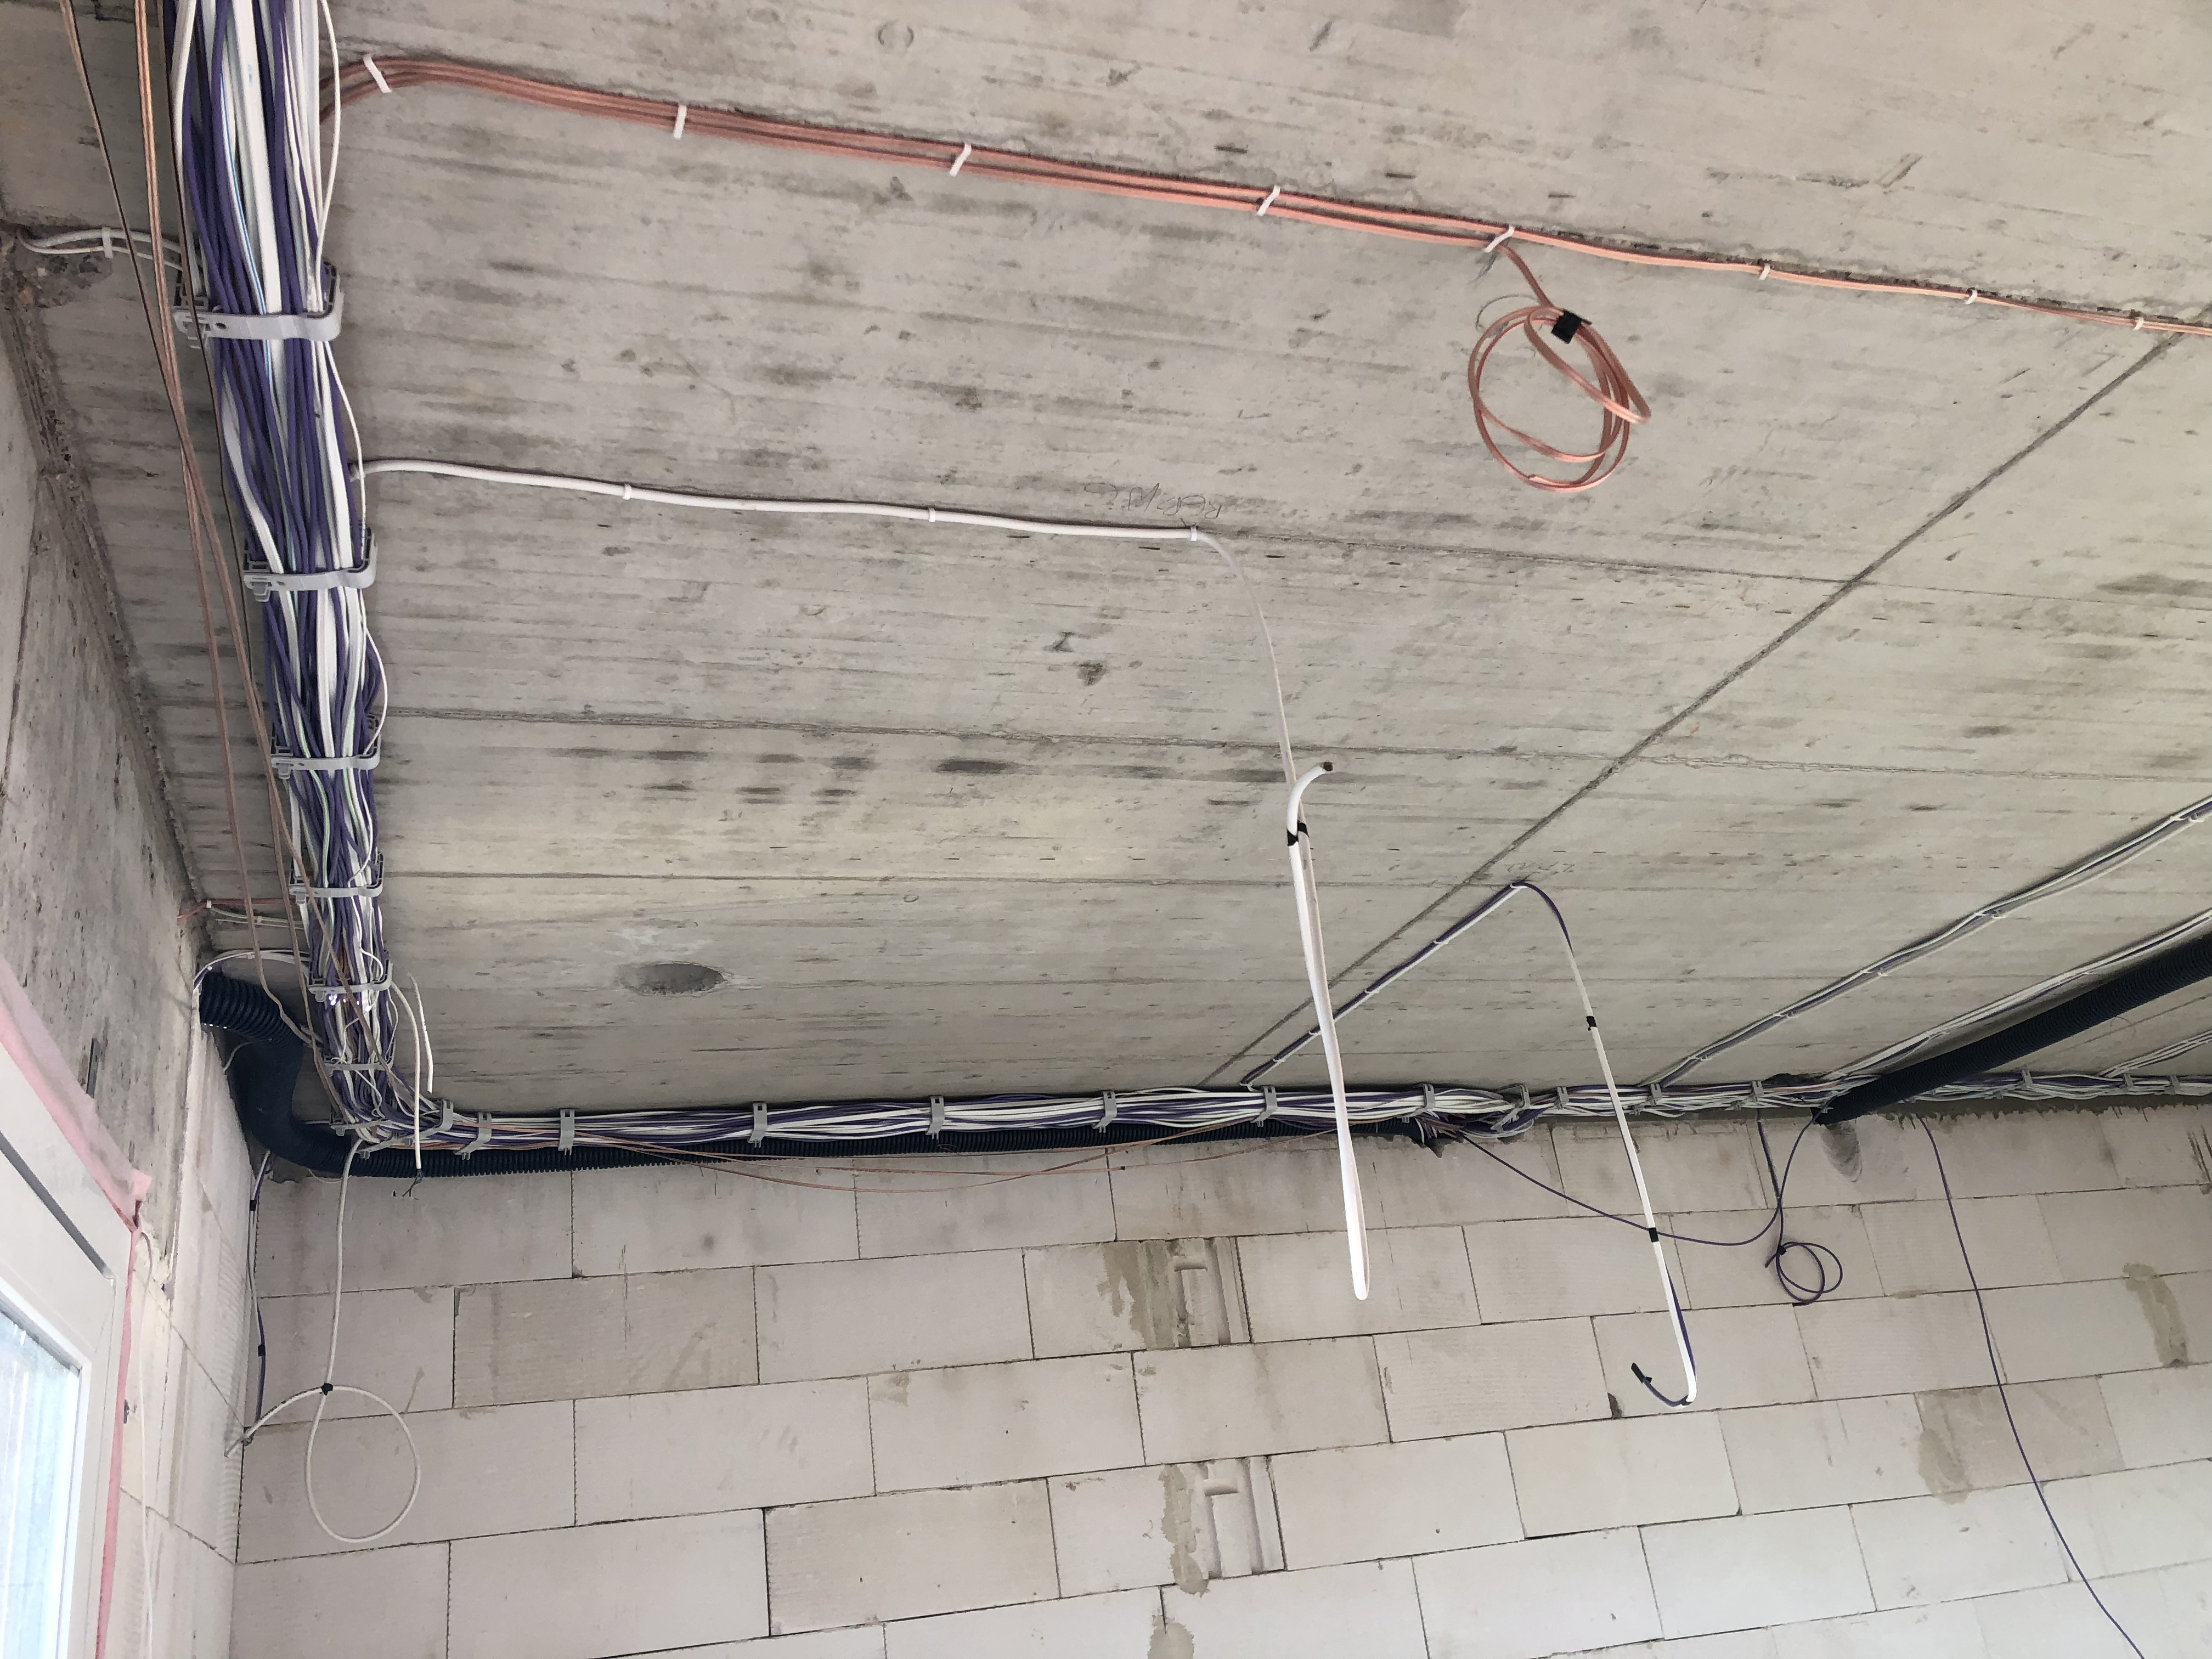
\includegraphics[width=0.8\columnwidth]{imgs/domkable.png}
\caption{Przykład okablowaniem domu inteligentnego. [źródło: materiały własne] \label{kable}}
\quad
\end{figure}

Żaden system nie posiada jednak wszystkich funkcjonalności, które są niezbędne danemu użytkownikowi. W większości z nich brakuje mobilnego systemu pozwalającego na rozpoznanie osób oraz podjęcia konkretnych działań w zależności od osoby, która została zidentyfikowana.

System inteligentnego rozpoznawania osób, który jest tematem niniejszego projektu, pozwala właśnie na identyfikację osób wchodzących do pomieszczenia na podstawie zapisanej wcześniej bazy zdjęć oraz powitanie ich indywidualnym komunikatem zarówno głosowym, jak i wizualnym.

Do realizacji projektu wykorzystałem \textcolor{red}{micro-komputer} Raspperry Pi 4B oraz język programowania Python 3. Jako elementu wejściowego sygnału użyłem kamery Raspberry Pi Camera HD v2 8MPx zgodnej z Raspperry Pi 4B, oraz najzwyklejszego głośnika pod wejscie jack 3,5mm

\subsection{Cel i zakres pracy}

Celem głównym projektu jest stworzenie prototypu inteligentnego, mobilnego systemu rozpoznawania osób, na podstawie wcześniej zgromadzonej bazy zdjęciowej, a także wygenerowanie unikatowego powitania głosowego oraz wizualnego w zależności od rozpoznanej osoby.

Celami szczegółowymi projektu są wybór technologii sprzętowej, wybór technologii programistycznej oraz zaprojektowanie i wykonanie obudowy prototypu, mieszczącej wszystkie elementy projektu

Praca swoim zakresem obejmuje zarówno tematykę z dziedziny elektroniki, informatyki projektowania oraz prototypowania 3D.

W zakresie elektroniki wykorzystane zostały układy i sensory zgodne z płytką Rasppery 4B, w zakresie informatyki napisany został program w języku Python 3 i wykorzystujący do realizacji zadań dostępne biblioteki, natomiast w zakresie prototypowania z wykorzystaniem druku 3D, użyta została drukarka 3D Creality Ender v2 oraz materiał \textcolor{red}{PET-G}. Do celów zaprojektowania obudowy wykorzystano program SOLIDWORKS. % w PET-G prototypuje, nie wiem czy starczy mi akurat tego materiału 

Projekt z jednej strony pokazuje, że połączenie wiedzy z zakresu elektroniki, informatyki oraz projektowania dostarcza każdemu studentowi odpowiednią wiedzę oraz umiejętności, do wykonania prototypu od fazy projektowej do fazy praktycznego zastosowania,  z drugiej udowadnia, że wiedza ta pozwala na wykonania projektu z wykorzystaniem elementów ogólnodostępnych na rynku.

\subsection{Struktura pracy} % tutorial jak prrace czytać

Rozdział pierwszy zawiera wstęp, wprowadzenie, opis celu oraz zakresu pracy, a także strukturę pracy. Znajdują się w nim podstawowe informacje opisujące główne elementy składowe projektu, oraz umożliwia szybkie zapoznania się z projektem na poziomie ogólnym

Rozdział drugi zawiera założenia odnośnie szczegółowych wymagań stawianych projektowi i umożliwia zrozumienie koncepcji projektu zarówno na poziomie ogólnym i bardziej szczegółowym.

Rozdział trzeci zawiera zestawienie założone funkcjonalności projektu, które będą zaimplementowane w projektowanym systemie oraz sposób korzystania z tych funkcjonalności.

Rozdział czwarty zawiera szczegółowy opis warstwy sprzętowej z wyszczególnieniem użytych w projekcie podzespołów oraz ich parametrów. Znajdują się w nim szczegółowe opisy użytej do projektu kamery, mikrokomputera Raspberry Pi, głośnika oraz ekranu służącego do komunikacji z użytkownikiem.

W rozdziale piątym znajduje się opis warstwy programistycznej projektu z uzasadnieniem wyboru języka Python jako języka programowania użytego w projekcie, opis zastosowanych bibliotek, algorytm oraz główne elementy kodu odpowiedzialne za działanie całego projektu.

W rozdziale szóstym znajduje się opis warstwy produktowej projektu z opisem użytej technologii druku 3D, kroków projektowania obudowy, procesu wykonania obudowy oraz szczegółów samej obudowy.

W rozdziale siódmym opisane zostały kwestie związane z samą realizacją projektu, napotkane problemy oraz sposoby jakimi problemy zostały rozwiązane. Omówiono także potencjalne możliwości rozbudowy projektu o kolejne funkcjonalności i zastosowania.

W rozdziale ósmym zawarto wnioski oraz „Lessons learned” z wykonanego projektu. Stanowią one podstawę do dalszego doskonalenia podejścia przy kolejnych projektach.

\newpage
\section{Wymagania stawiane projektowi}

W celu realizacji pracy w pierwszej kolejności zostały określone wymagania, które stanowiły punkt docelowy projektu, jaki należało osiągnąć w ramach prac projektowych, a następnie pozwoliły na zaplanowanie drogi dojścia do założonego celu.

Na podstawie założonego celu zostały określone kroki milowe, które należało osiągnąć. Kroki te dzieliły cały projekt na mniejsze etapy, z jednej strony pozwalające na lepszy nadzór nad postępami pracy, oraz natychmiastowe określenie punktów stanowiących problem i wstrzymujących postępy, a z drugiej strony pozwalały na elastyczne reagowanie i zmiany projektowe bez konieczności zmian poprzednich etapów.

Takie podejście miało zapewnić iż ewentualny błąd popełniony na dalszych etapach nie będzie miał wpływu na etapy poprzednie projektu.

\begin{figure}[!ht]%
\centering
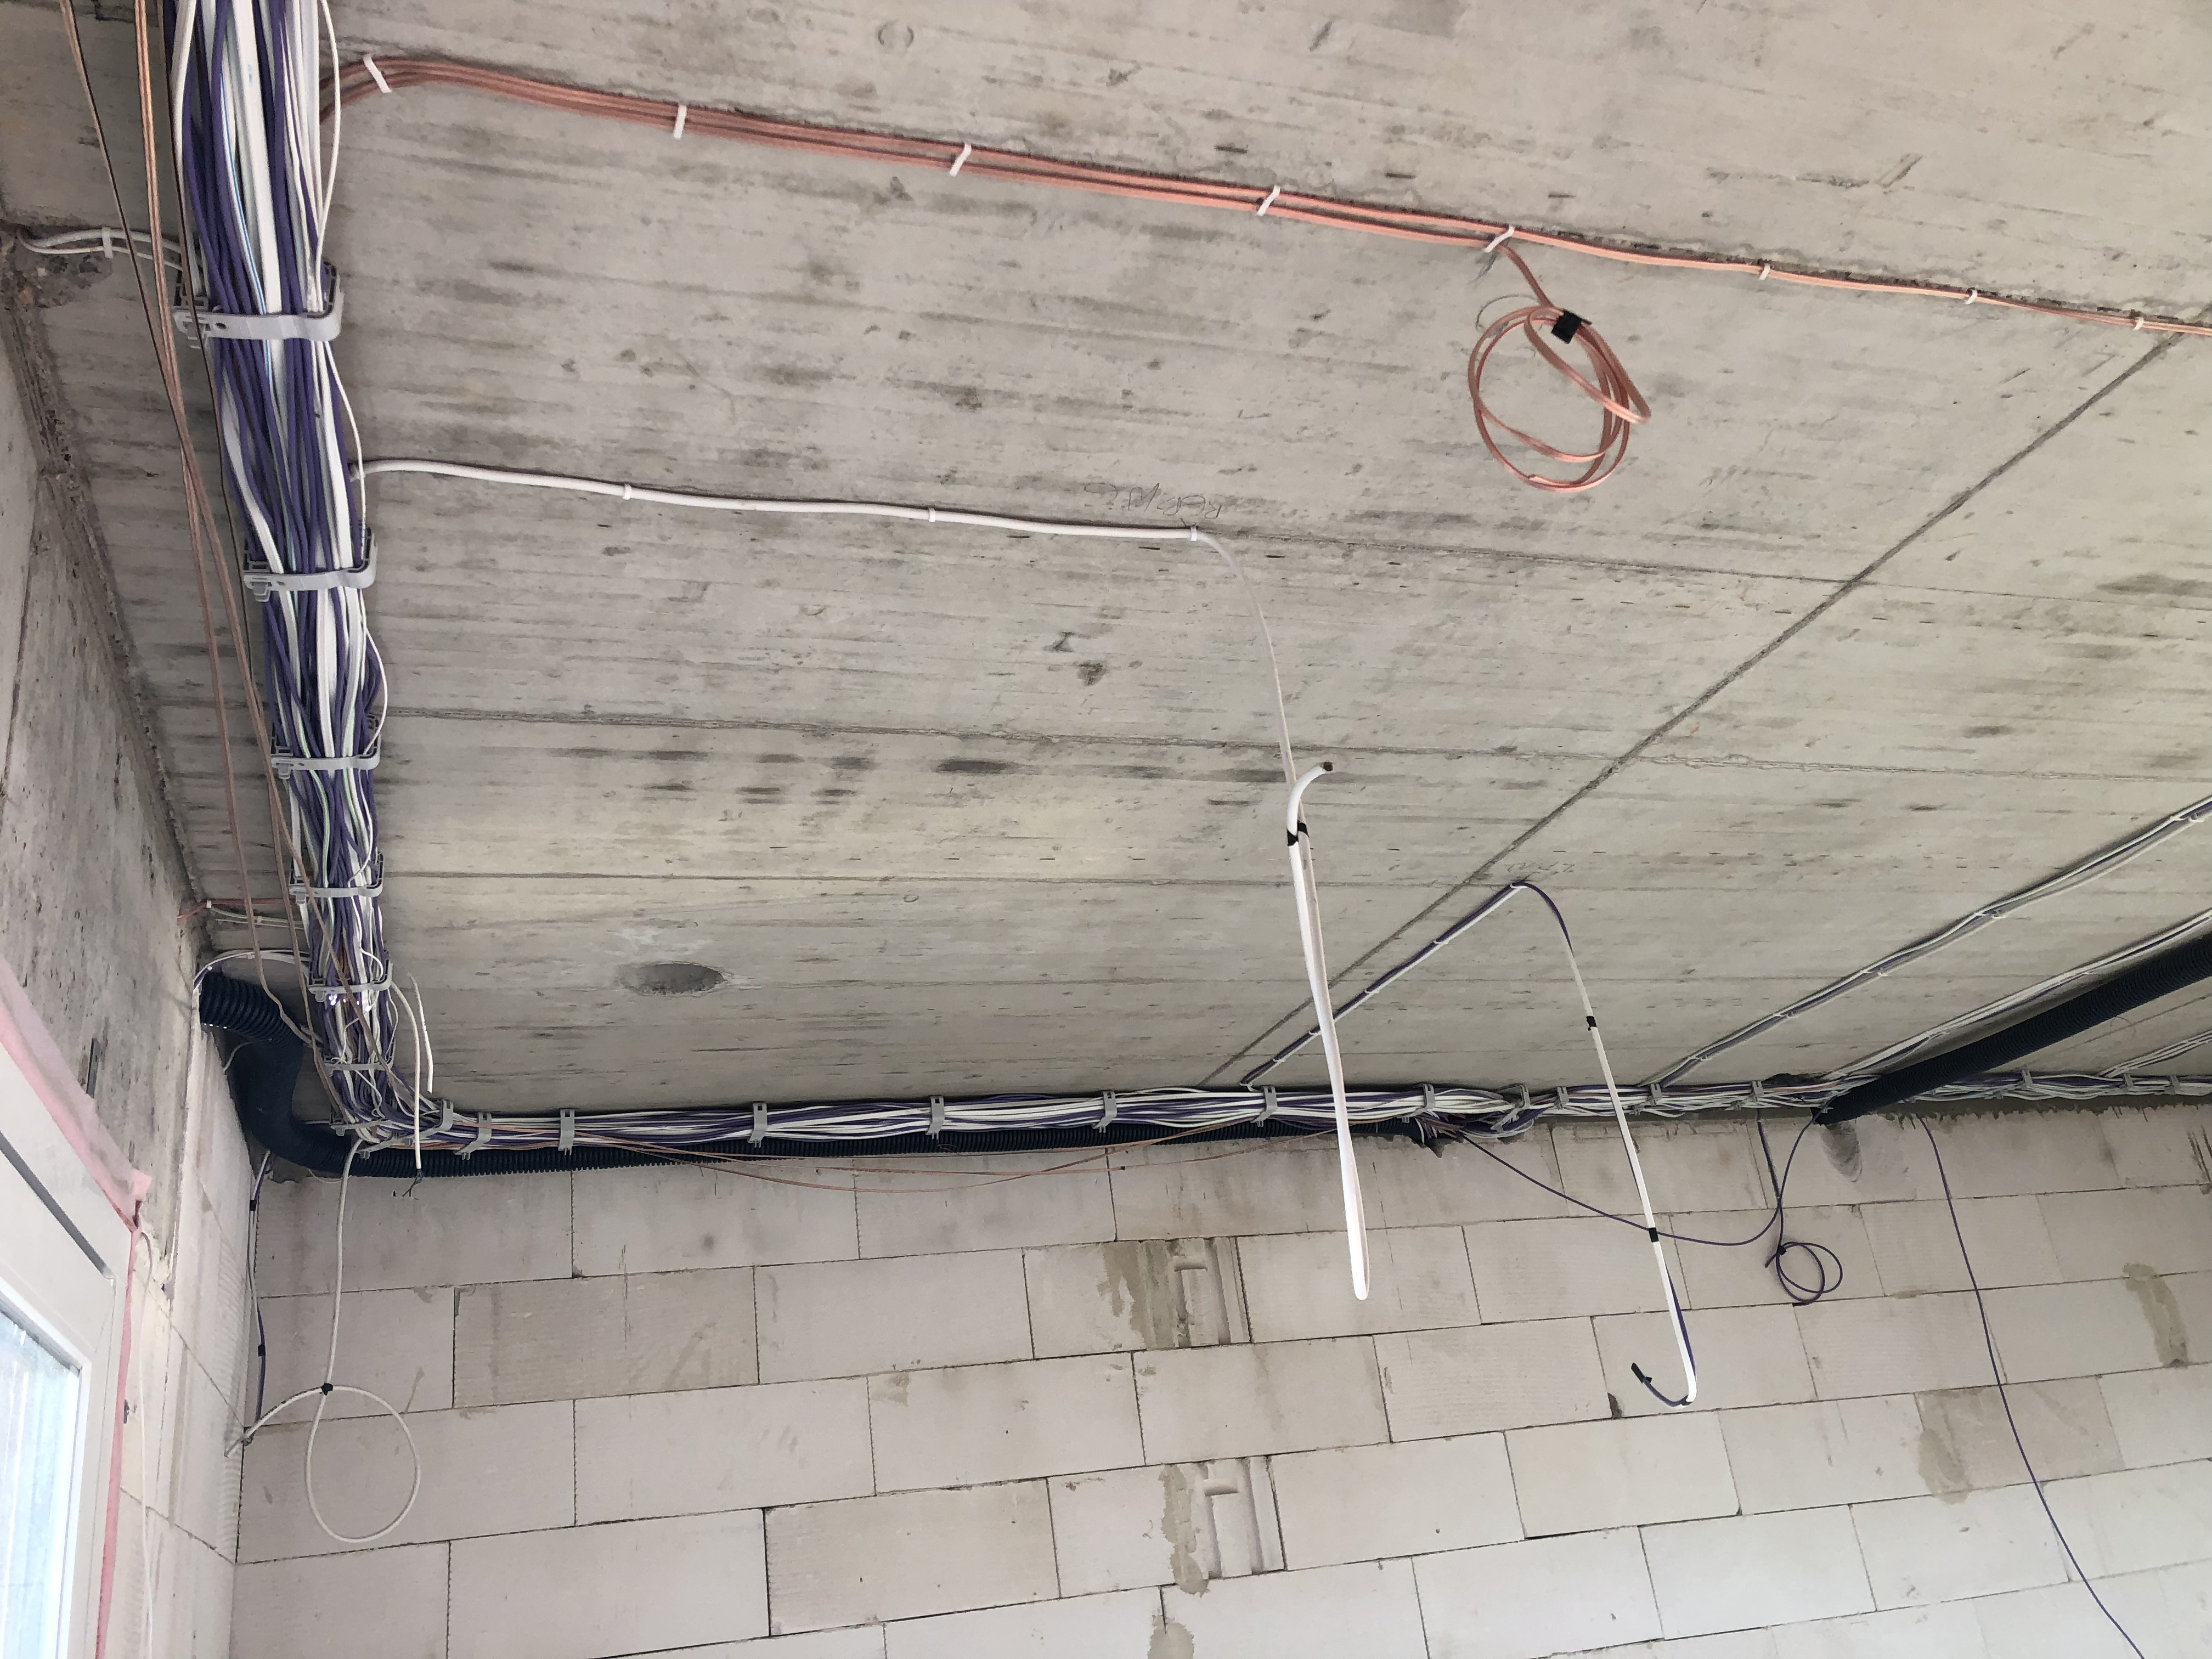
\includegraphics[width=0.8\columnwidth]{imgs/domkable.png}
\caption{Etapy prac projektowych. [źródło: opracowanie własne] \label{etapypracy}}
\quad
\end{figure}

\subsection{Wymagania dla prototypu}

W ramach realizacji projektu zostały określone następujące wymagania dla prototypu.

\begin{itemize}
	\item \textbf{Mobilność.} Głównym założeniem projektu jest mobilność prototypu. Oznacza to, iż będzie posiadał wymiary oraz wagę umożliwiającą łatwe przenoszenie w dowolne miejsce.
	\item \textbf{Łatwość zasilania.} Prototyp powinien mieć możliwość zasilania z ogólnodostępnej sieci 230V, tak aby istniała możliwość stałego podłączenia do gniazda elektrycznego. Opcjonalnie założono, że prototyp będzie posiadał możliwość podłączenia do zasilania z baterii lub akumulatorów, tak aby mógł znaleźć zastosowanie w miejscach, w których dostęp do sieci elektrycznej jest utrudniony.
	\item \textbf{Dostępność.} Prototyp zostanie wykonany ze standardowych elementów dostępnych na rynku polskim.
	\item \textbf{Relatywnie niski koszt.} Wykonanie prototypu powinno mieścić się w kwocie nie większej niż \textcolor{blue}{1000zł?}
	\item \textbf{Łatwość obsługi.} Prototyp będzie umożliwiał obsługę bez konieczności znajomości zagadnień technicznych. Zadaniem użytkownika będzie jedynie wprowadzenie bazy zdjęć do określonego folderu, \textcolor{red}{odpalenia dwóch programów (program "zapisujący" zjęcia twarzy do zakodowanego pliku, główny program rozpoznający przechodniów)} i odpowiednie nakierowanie kamery prototypu.
	\item \textbf{Łatwość rozbudowy.} Platforma na jakiej zostanie zbudowany prototyp będzie pozwalała na jego łatwą rozbudowę.
	\item \textbf{Łatwość programowania.} System będzie oparty o jeden z popularnych języków programowania, w którym dostępne są biblioteki niezbędne do realizacji wszystkich zadań, tak aby użytkownik mógł skorzystać z dostępnych standardowych rozwiązań programistycznych, bez ponoszenia dodatkowych kosztó
\end{itemize}

\subsection{Wymagania dla procesu projektowego}

W celu wykonania prototypu zostały określone następujące wymagania dla procesu projektowego.

\begin{itemize}
	\item \textbf{Elastyczność.} Projekt zostanie podzielony na mniejsze etapy, tak aby w każdej chwili istniała możliwość modyfikacji założeń lub działań przy jednoczesnym zapewnieniu realizacji założonych celów.
	\item \textbf{Dostępność narzędzi.} Dla każdego etapu projektu zostaną użyte narzędzia dostępne na rynku, tak aby uniknąć konieczności projektowania samych narzędzi.
	\item \textbf{Przejrzystość.} Na każdym etapie status prac będzie łatwo weryfikowalny aby zidentyfikować potencjalne przeszkody mogące powodować opóźnienie realizacji projektu.
	\item \textbf{Bezpieczeństwo.} \textcolor{red}{W celu uniknięcia utraty danych zostanie wykorzystane repozytorium Git, a dodatkowo dane będą zapisywane na komputerze lokalnym.}
\end{itemize}

\newpage
\section{Oczekiwane funkcjonalności projektu}

W ramach realizacji projektu zostały zaimplementowane następujące funkcjonalności.

\begin{itemize}
	\item \textcolor{red}{\textbf{Zencodowanie znanych twarzy.} Użytkownik do imiennych folderów wprowadza zdjęcia osoby (np. Zdjęcia Jana wrzucam do folderu "Jan Nowak") i odpala program encodujący zamieniając twarz na wartości liczbowe.}
	\item \textcolor{red}{\textbf{Użycie syntezatora mowy.}} System korzysta z syntezatora mowy w celu \textcolor{red}{dodania deflautowego powitania do pliku .mp3.}
	\item \textbf{Wykrycie osoby.} System skanuje wybrany obszar przestrzeni i wykrywa czy w nadzorowanym obszarze znajduje się osoba. W przypadku wykrycia aktywowane są kolejne algorytmy programu. System pomija zwierzęta oraz przedmioty.
	\item \textbf{Skanowanie  twarzy.} Po wykryciu obiektu kamera koncentruje się na twarzy wykrytej osoby i \textcolor{red}{encoduje w celu porównania z lokalną bazą.}
	\item \textbf{Porównanie \textcolor{red}{(Identyfikacja)} twarzy.} \textcolor{red}{System porównuje nasze zencodowane zdjęcie z wcześniej zencodowanymi zdjęciami bazowymi, jeśli znalazło taki sam hasz, to znalazło osobę.}
	\item \textbf{Komunikat głosowy.} \textcolor{red}{Z puli powitań plików \textcolor{blue}{.mp3} (deflautowo jeden, można wrzucić własne dzwięki), program losuje jeden i go odpala \textcolor{blue}{(W przypadku gdy jest tylko jeden plik, losowanie się nie odbywa)}.}
	\item \textbf{Komunikat wizualny.} \textcolor{red}{Na ekranie dodatkowo pojawia się komunikat graficzny \textcolor{blue}{z imieniem i nazwiskiem}. W przypadku wykrycia osoby nieznanej pojawia się stosowny komunikat (Patrz rys. \ref{komunikatgraficzny:komunikatgraficzny}\subref{komunikatgraficzny:1}, \ref{komunikatgraficzny:komunikatgraficzny}\subref{komunikatgraficzny:2})}
\end{itemize}
\begin{figure}[!ht]%
	\centering
	\begin{subfigure}{.5\textwidth}
		\centering
		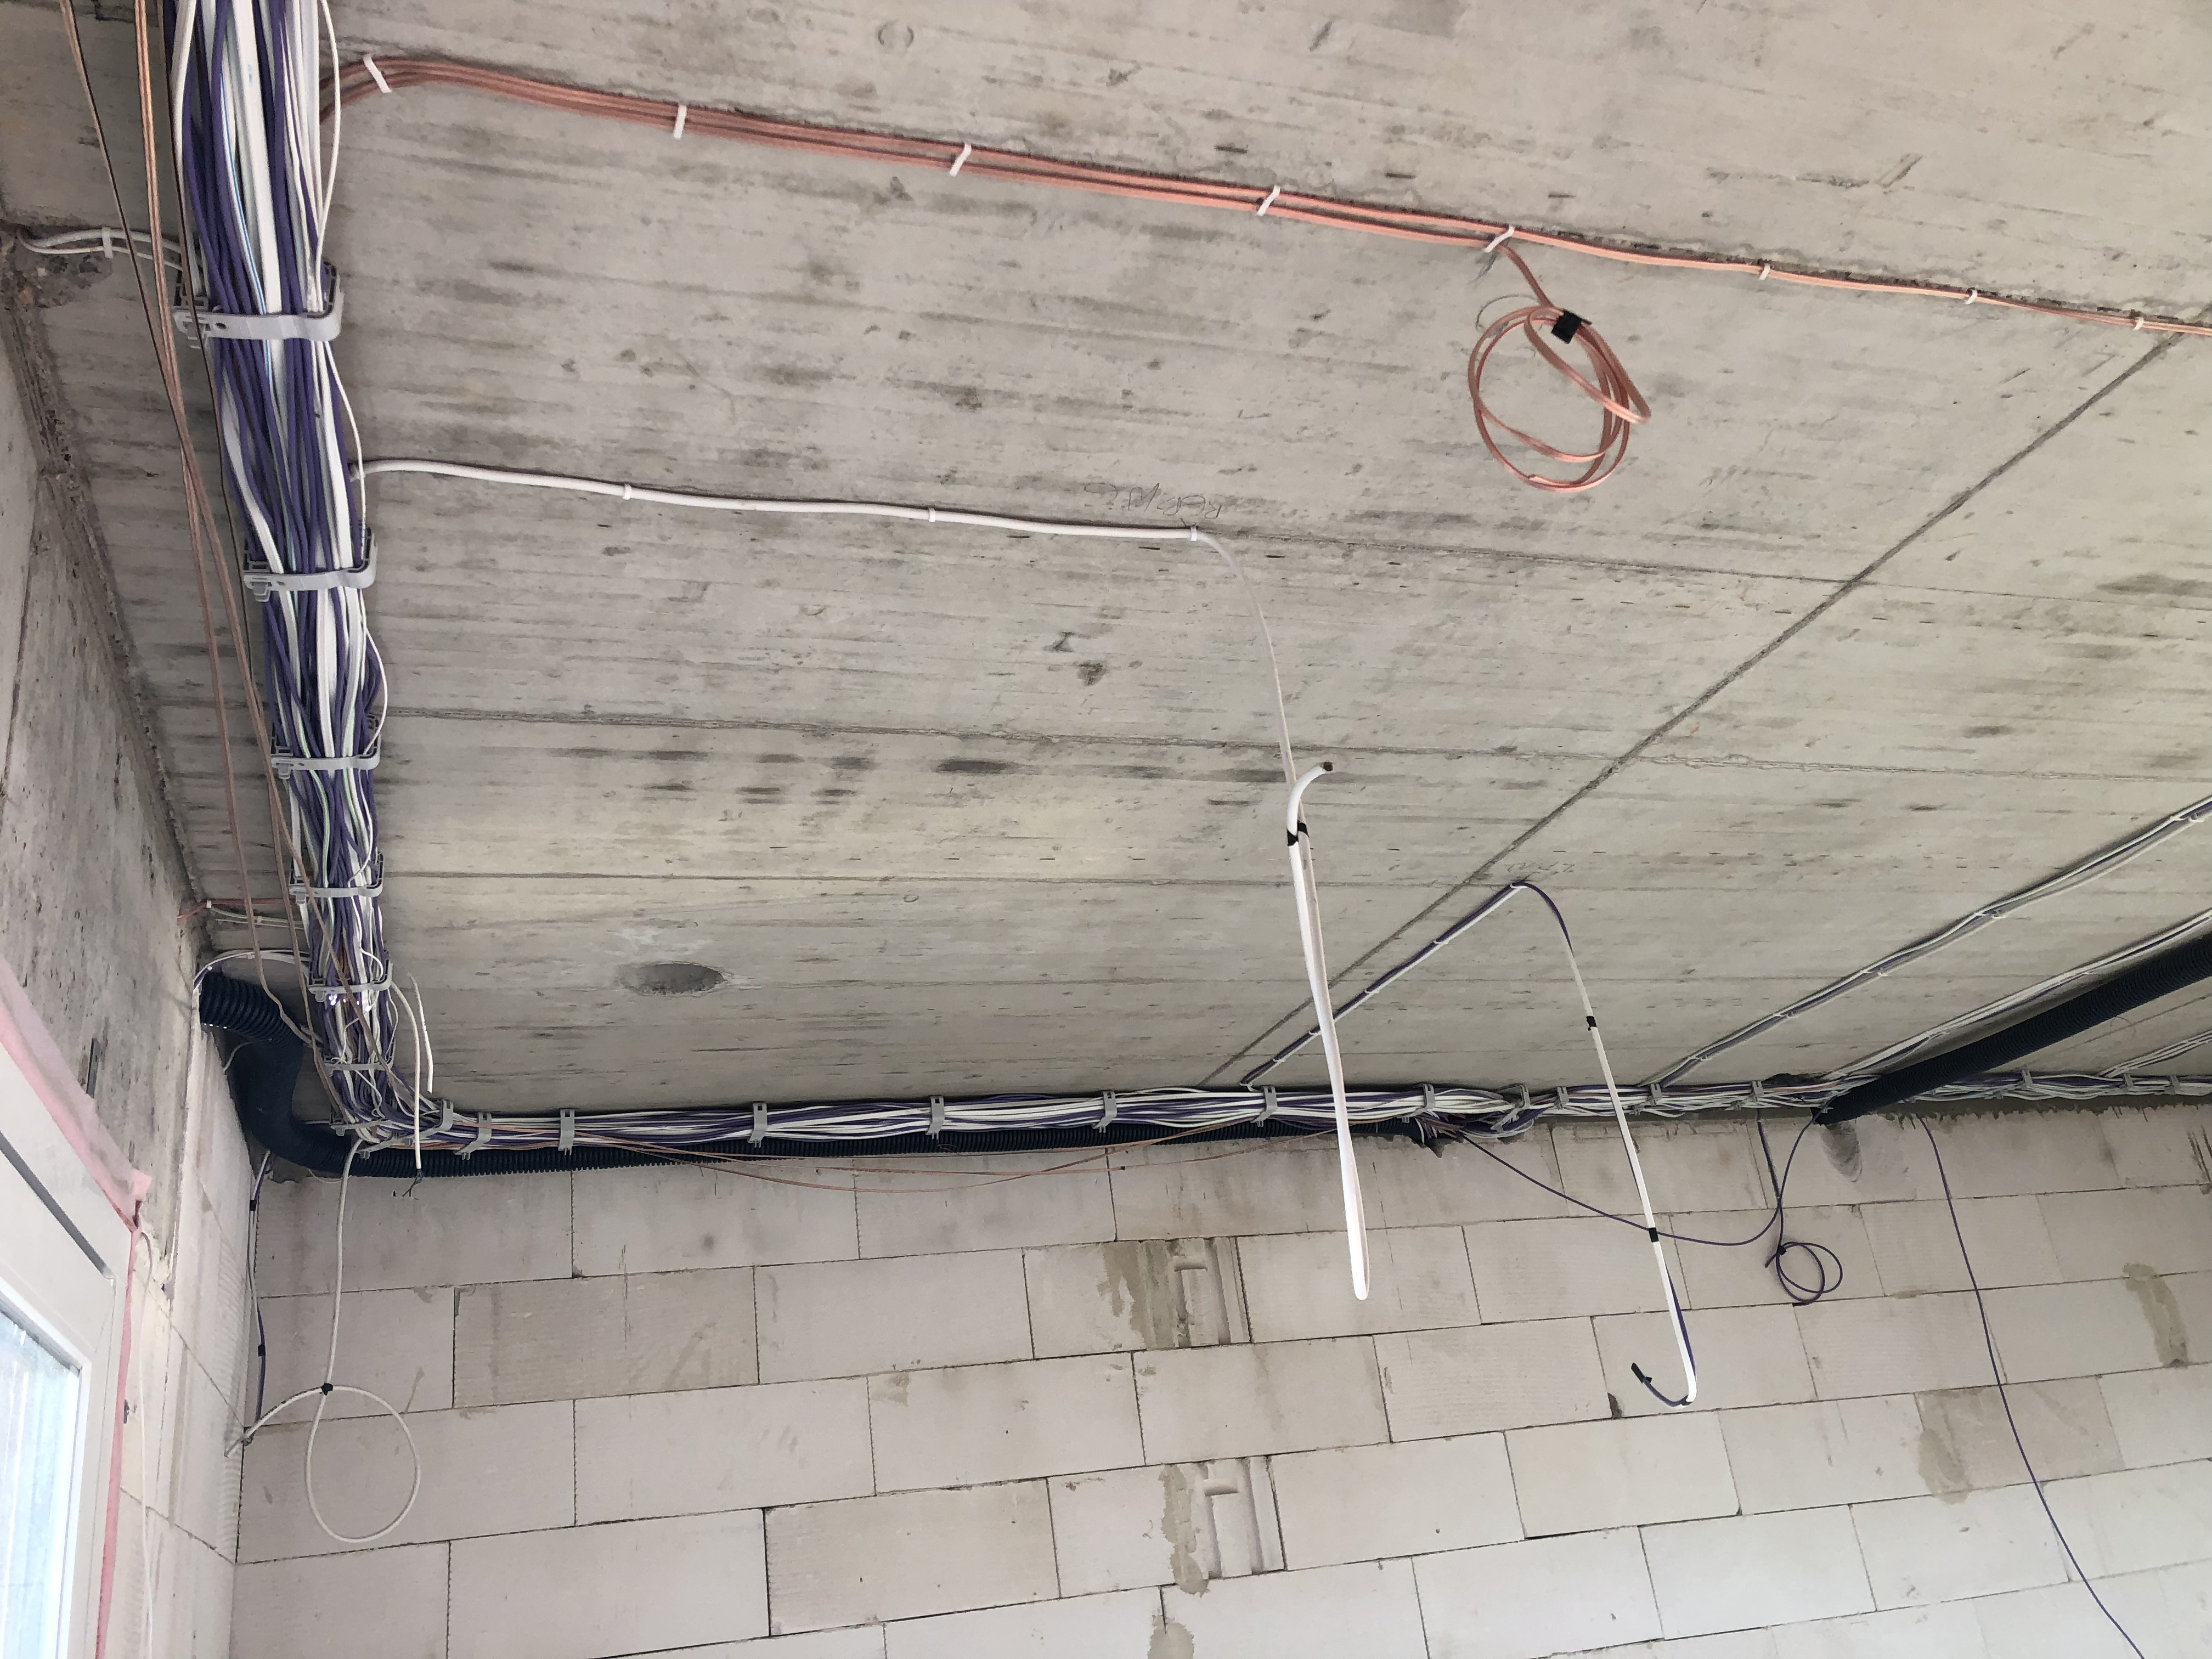
\includegraphics[width=0.8\linewidth]{imgs/domkable.png}
		\caption{Rozpoznanej osoby.}	
		\label{komunikatgraficzny:1}
	\end{subfigure}%
	\begin{subfigure}{.5\textwidth}
		\centering
		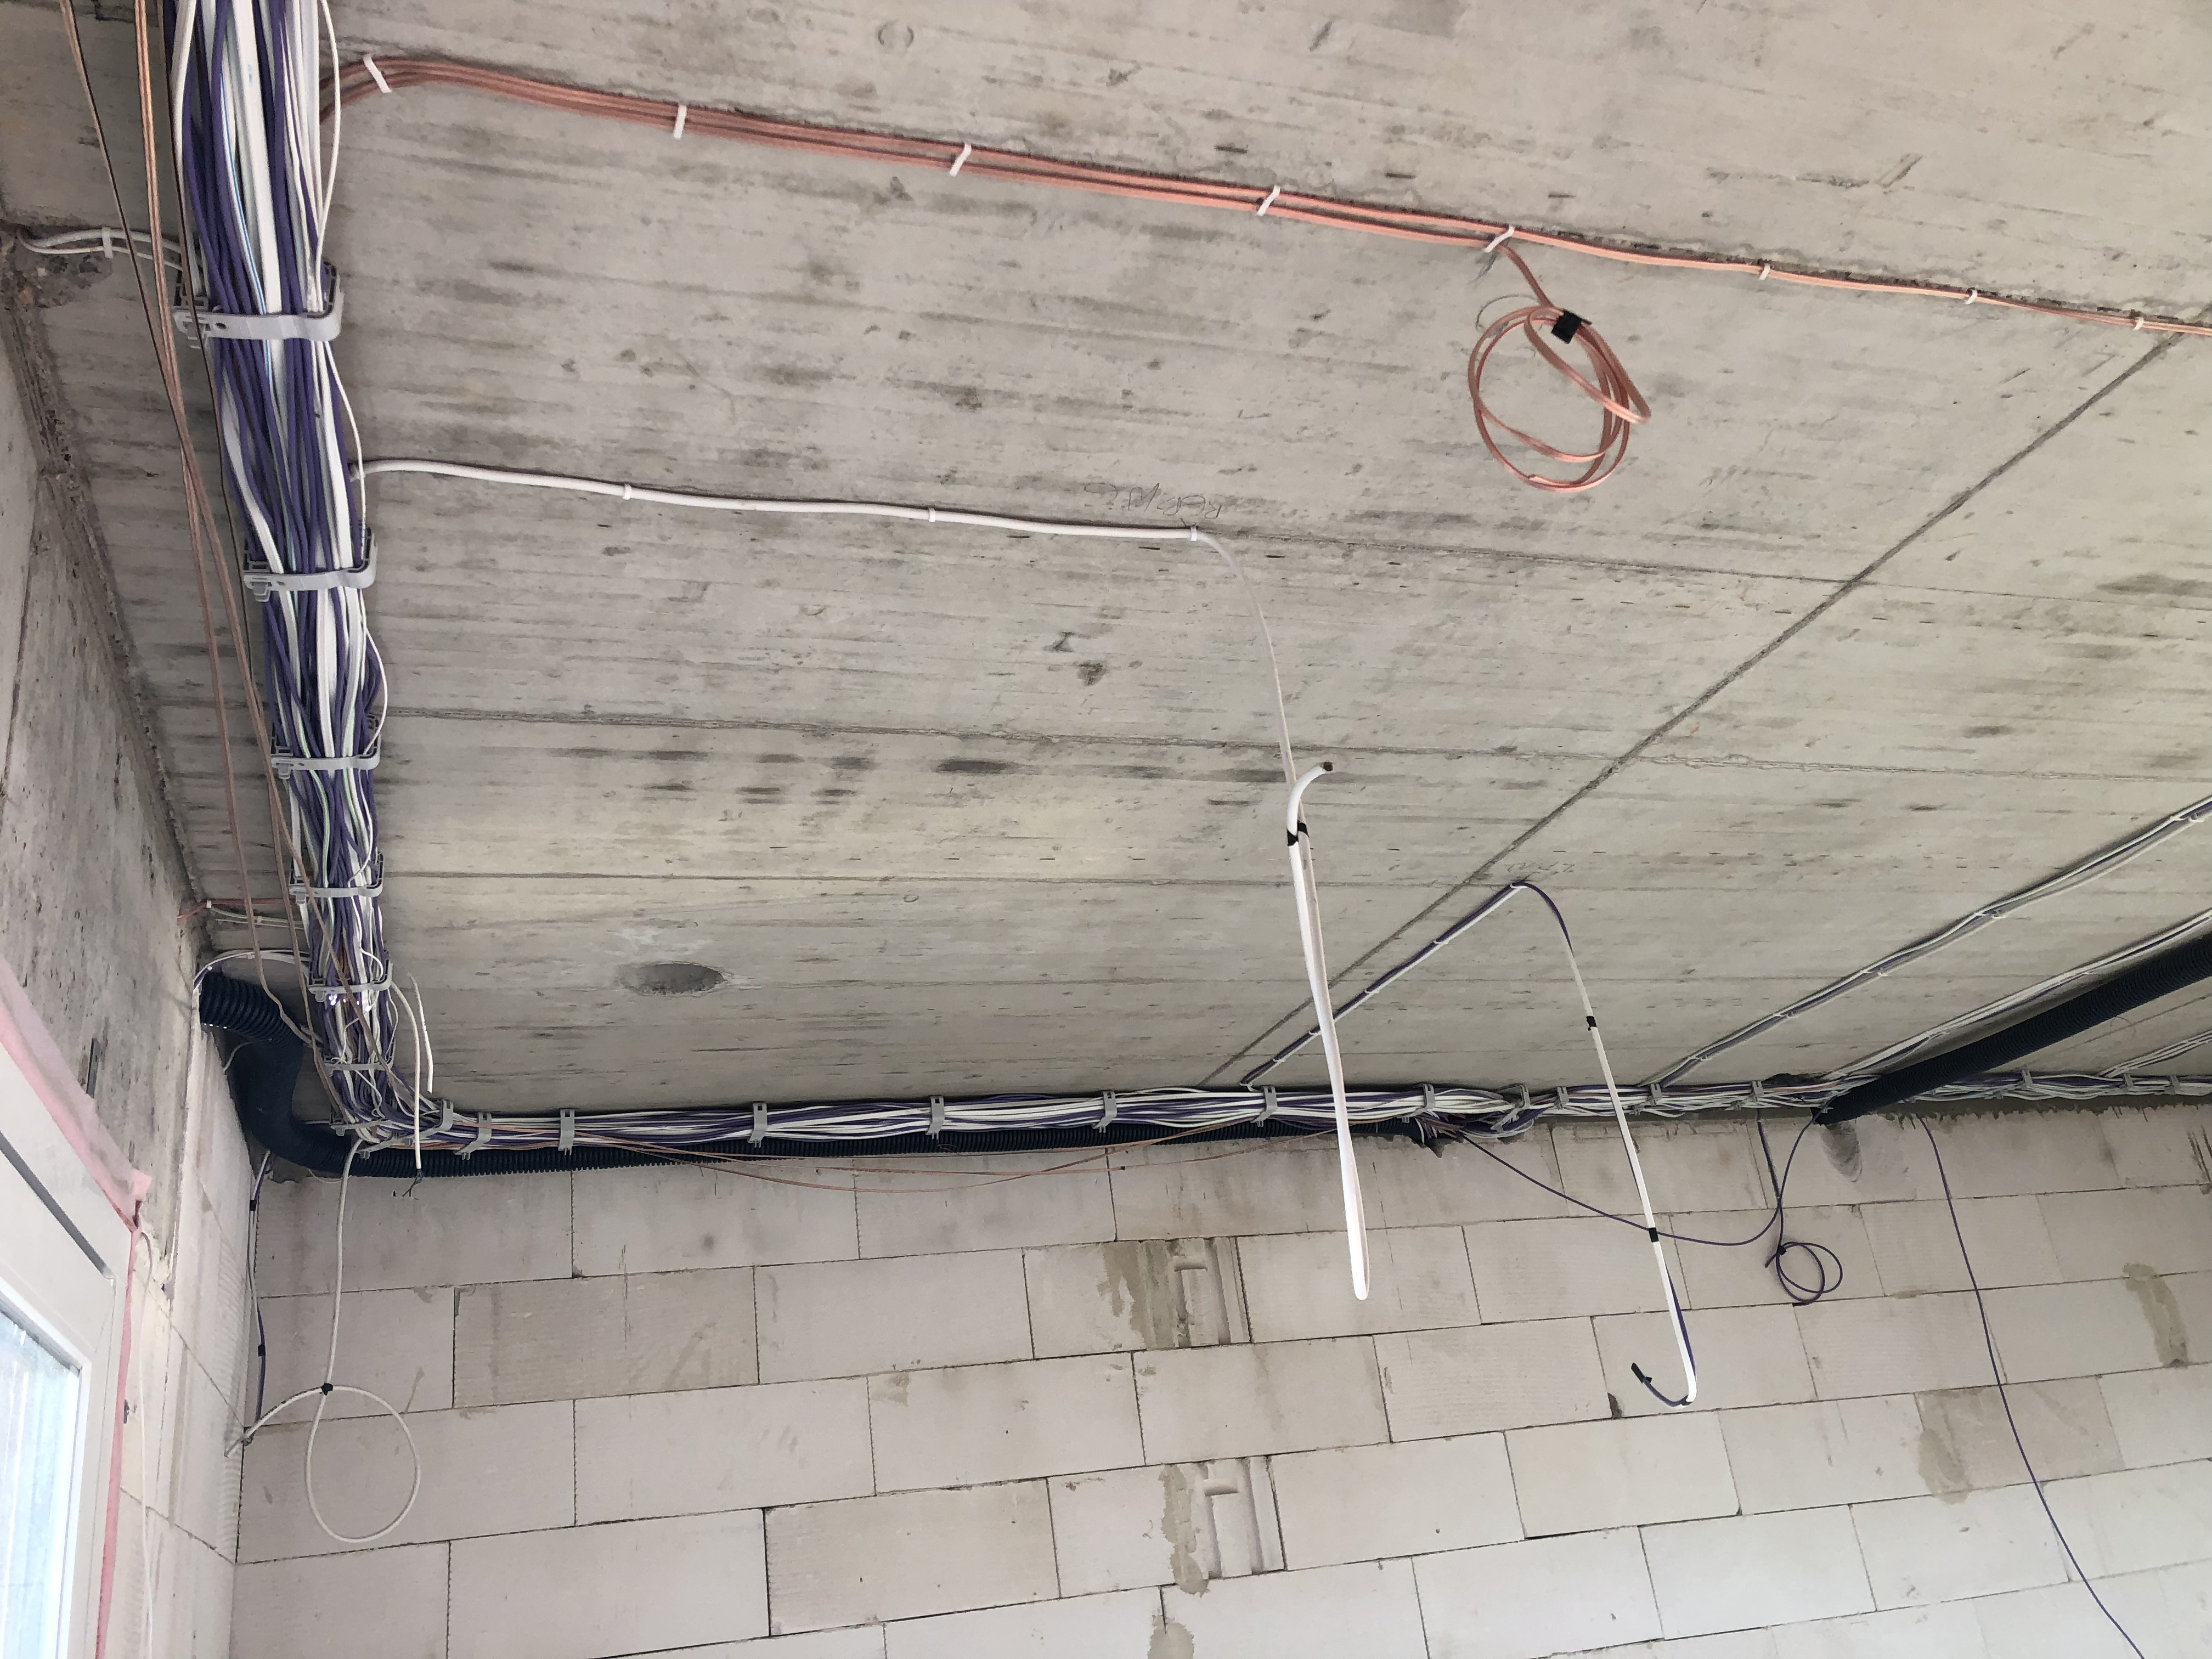
\includegraphics[width=0.8\linewidth]{imgs/domkable.png}
		\caption{NIE rozpoznanej osoby}
		\label{komunikatgraficzny:2}
	\end{subfigure}%
\caption{Komunikaty graficzne}
\label{komunikatgraficzny:komunikatgraficzny}
\end{figure}

Powyższe funkcjonalności pozwalają na realizację funkcji

\begin{itemize}
	\item powitania
	\item nadzór\textcolor{red}{?}
\end{itemize}

Przykłady realizacji funkcji powitania:

\begin{itemize}
	\item "Cześć Krzysiek, miło Cię widzieć"
	\item \textcolor{red}{"Witaj Krzysztof Kukiz"}
	\item \textcolor{red}{"Witaj w domu Krzysiek"}
	\item "Dzień dobry, zapraszamy do recepcji na pierwszym piętrze. Winda jest po prawej stronie"
\end{itemize}

\newpage
\section{Warstwa sprzętowa}

W ramach warstwy sprzętowej projekt składa się z 4 elementów. Kamery, mirko-komputera Raspberry Pi, głośnika oraz ekranu.

Podstawą systemu jest Raspberry Pi, do którego podłączone są wszystkie elementy wejściowe oraz wyjściowe prototypu, tak aby stanowiły spójną całość. W ten sposób przygotowana warstwa sprzętowa będzie następnie oprogramowana (patrz rozdział \textcolor{blue}{5}) oraz zabezpieczona obudową (patrz rozdział \textcolor{blue}{6})

\subsection{Kamera jako element wejściowy}

Spośród dostępnych kamer w projekcie zastosowano kamerę  HD v2 8MPx dedykowaną do mikrokomputera Raspberry Pi. Urządzenie posiada matrycę o rozdzielczości 8 Mpx, wspiera tryb HD 1080p, 720p oraz 640 x 480p oraz jest w stanie wykonywać zdjęcia w wyższej rozdzielczości 3280 x 2464 px.

Aby uniknąć potencjalnych problemów w przesyle sygnału zastosowano oficjalny moduł Raspberry Pi Camera HD v2, który jest całkowicie zgodny ze sterownikami, dostarczanymi wraz z systemem Raspberry Pi OS.

Dzięki takiemu rozwiązaniu możliwe jest jednocześnie szerokie wsparcie w zakresie dokumentacji, tutoriali oraz bibliotek programistycznych.

\textcolor{red}{Dostępne są także programy konsolowe do obsługi różnych trybów pracy kamery.}

\begin{figure}[!ht]%
\centering
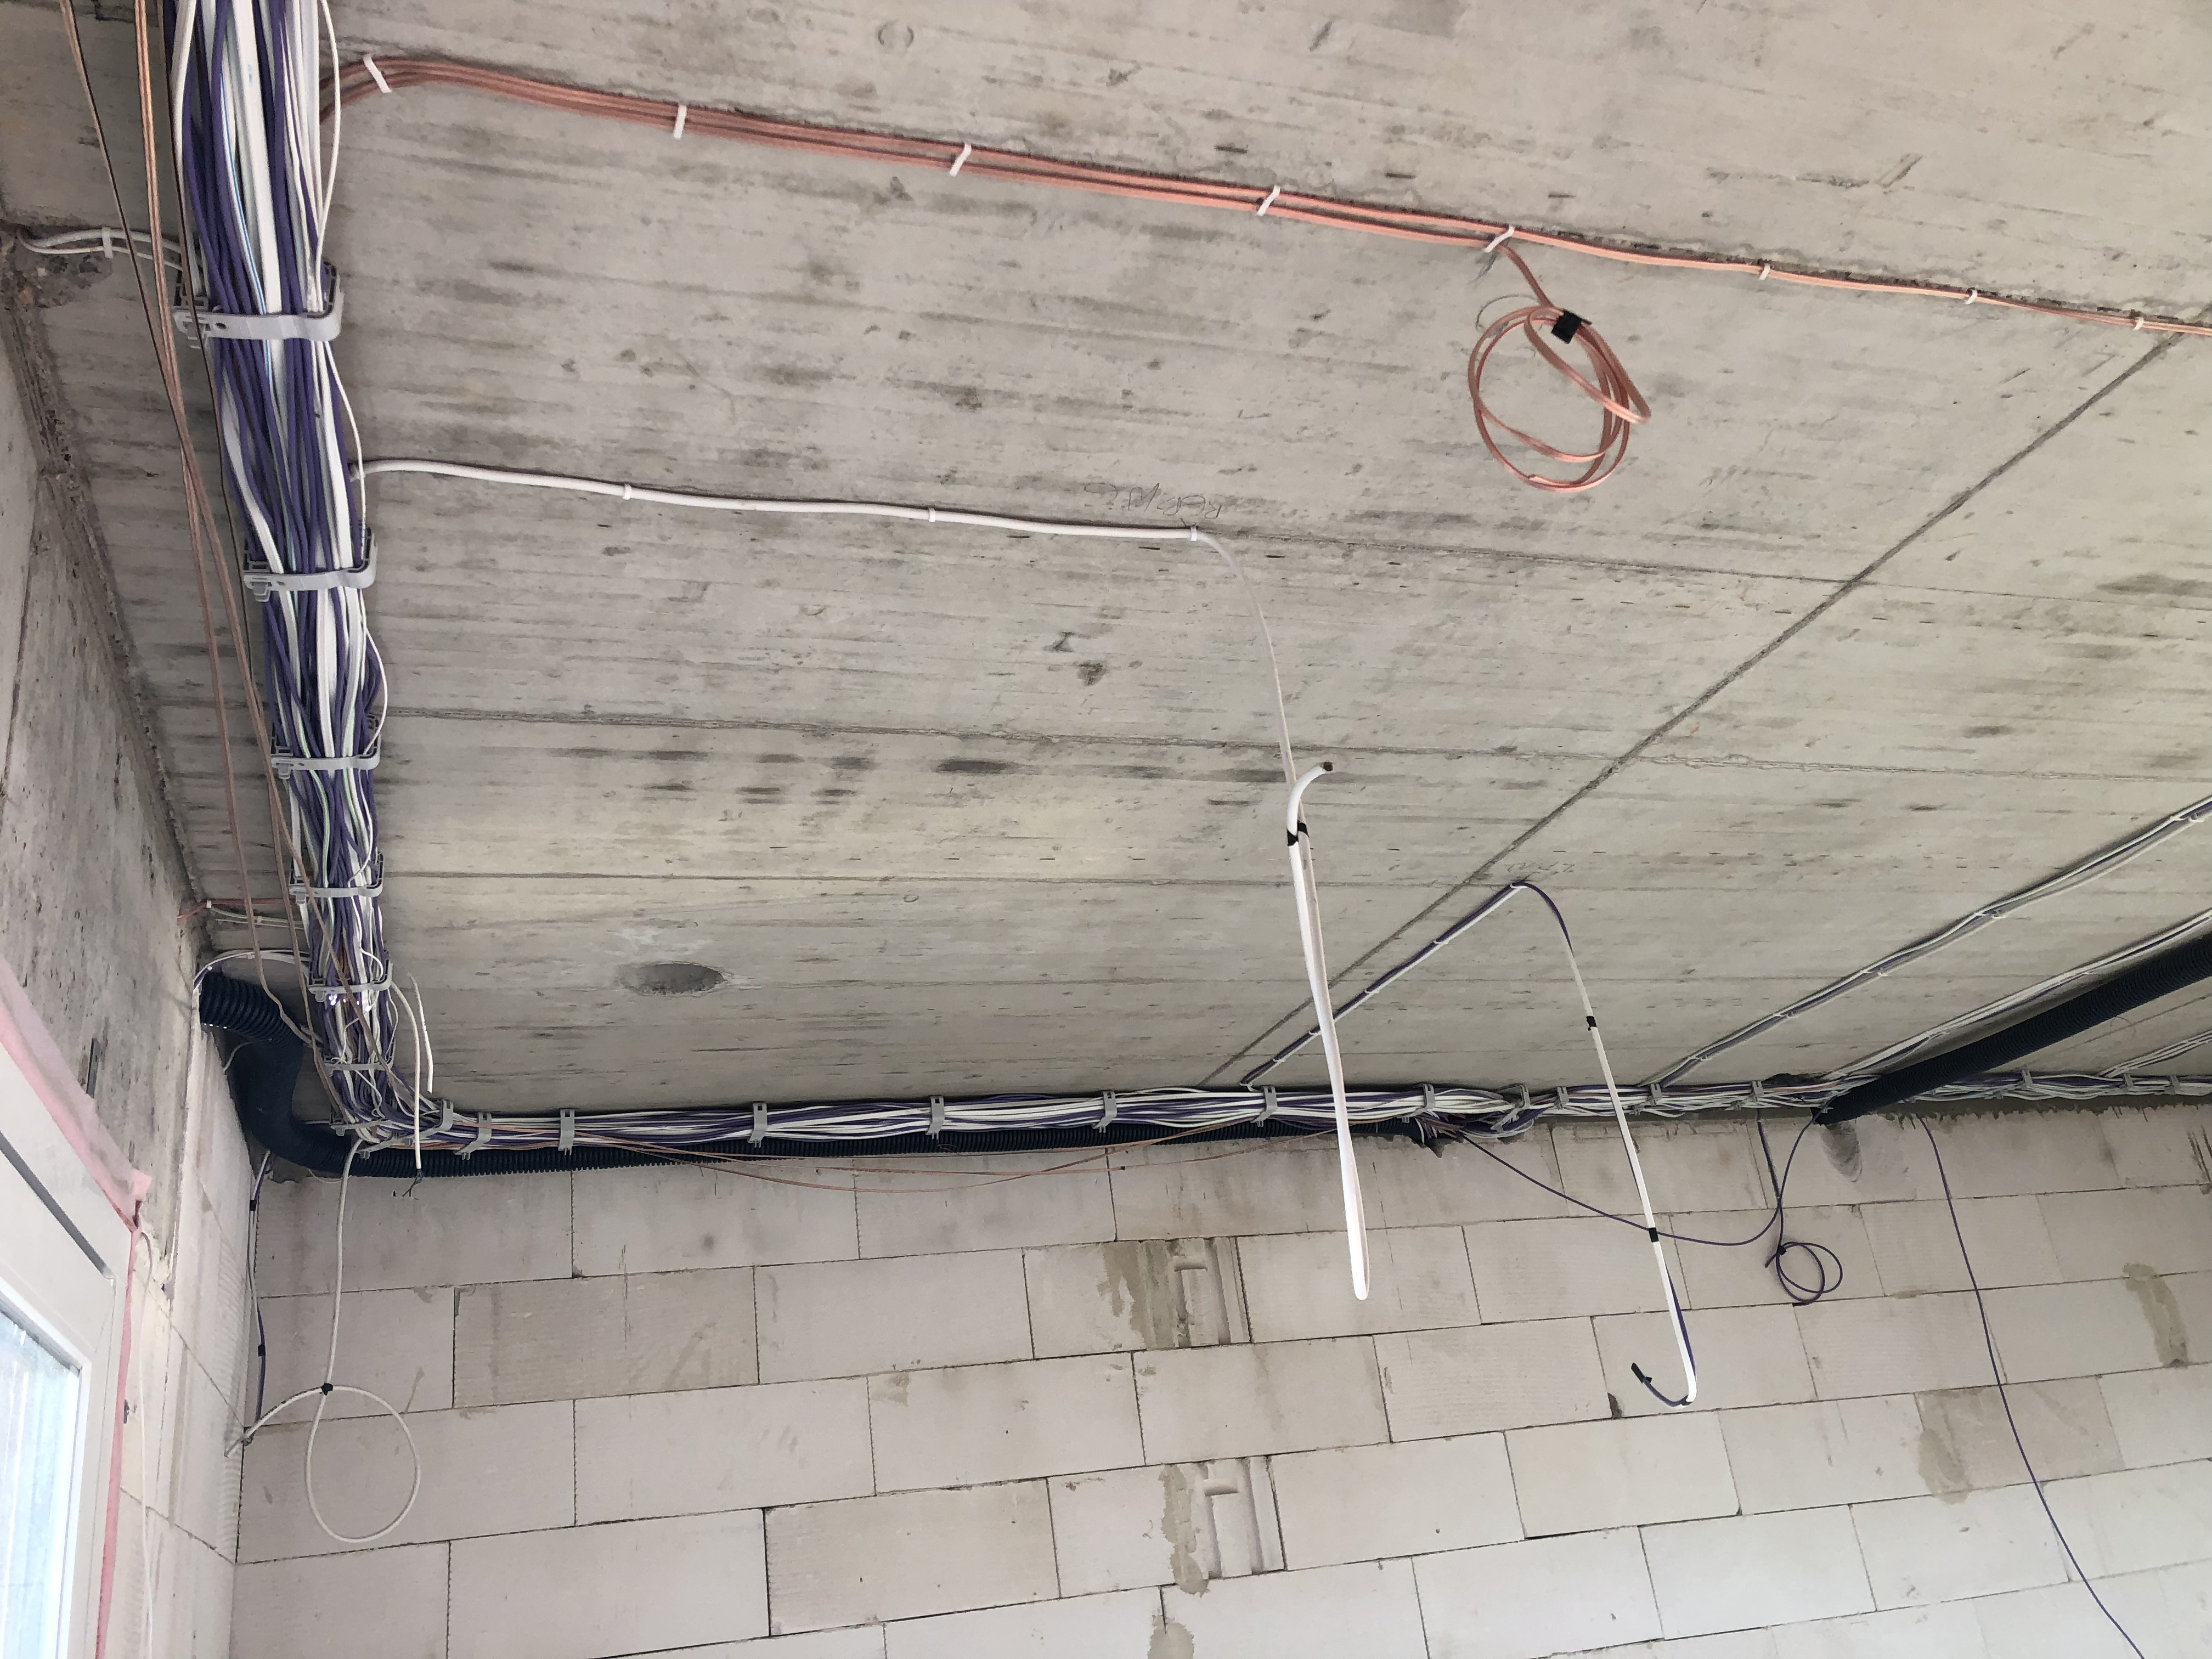
\includegraphics[width=0.8\columnwidth]{imgs/domkable.png}
\caption{Zdjęcie x. Kamera HD [źródło: ] \label{kamera}}
\quad
\end{figure}

Parametry kamery

\begin{itemize}
	\item HD 1080p / 30 fps,
	\item 720p / 60 fps,
	\item 640 x 480p / 90 fps.
\end{itemize}

\subsection{Płyta Raspberry Pi}

Spośród dostępnych modeli Raspberry Pi do projektu wykorzystano model w wersji 4B, który charakteryzuje się zwiększoną pojemnością pamięci RAP (4GB) oraz wydajniejszym procesorem (Broadcom BCM2711) quad-core 64-bitowy ARM-8.

Posiada on dwa złącza microHDMI, dwa złączami USB 3.0 i 2 złącza USB 2.0. Zasilanie realizowane jest przez złącze USB C.

Mikrokomputer wyposażony jest także w dwuzakresowe WiFi 2,4 GHz i 5 GHz, Bluetooth w standardzie 5, oraz port Ethernet o prędkości do 1000 Mb/s.

\begin{figure}[!ht]%
\centering
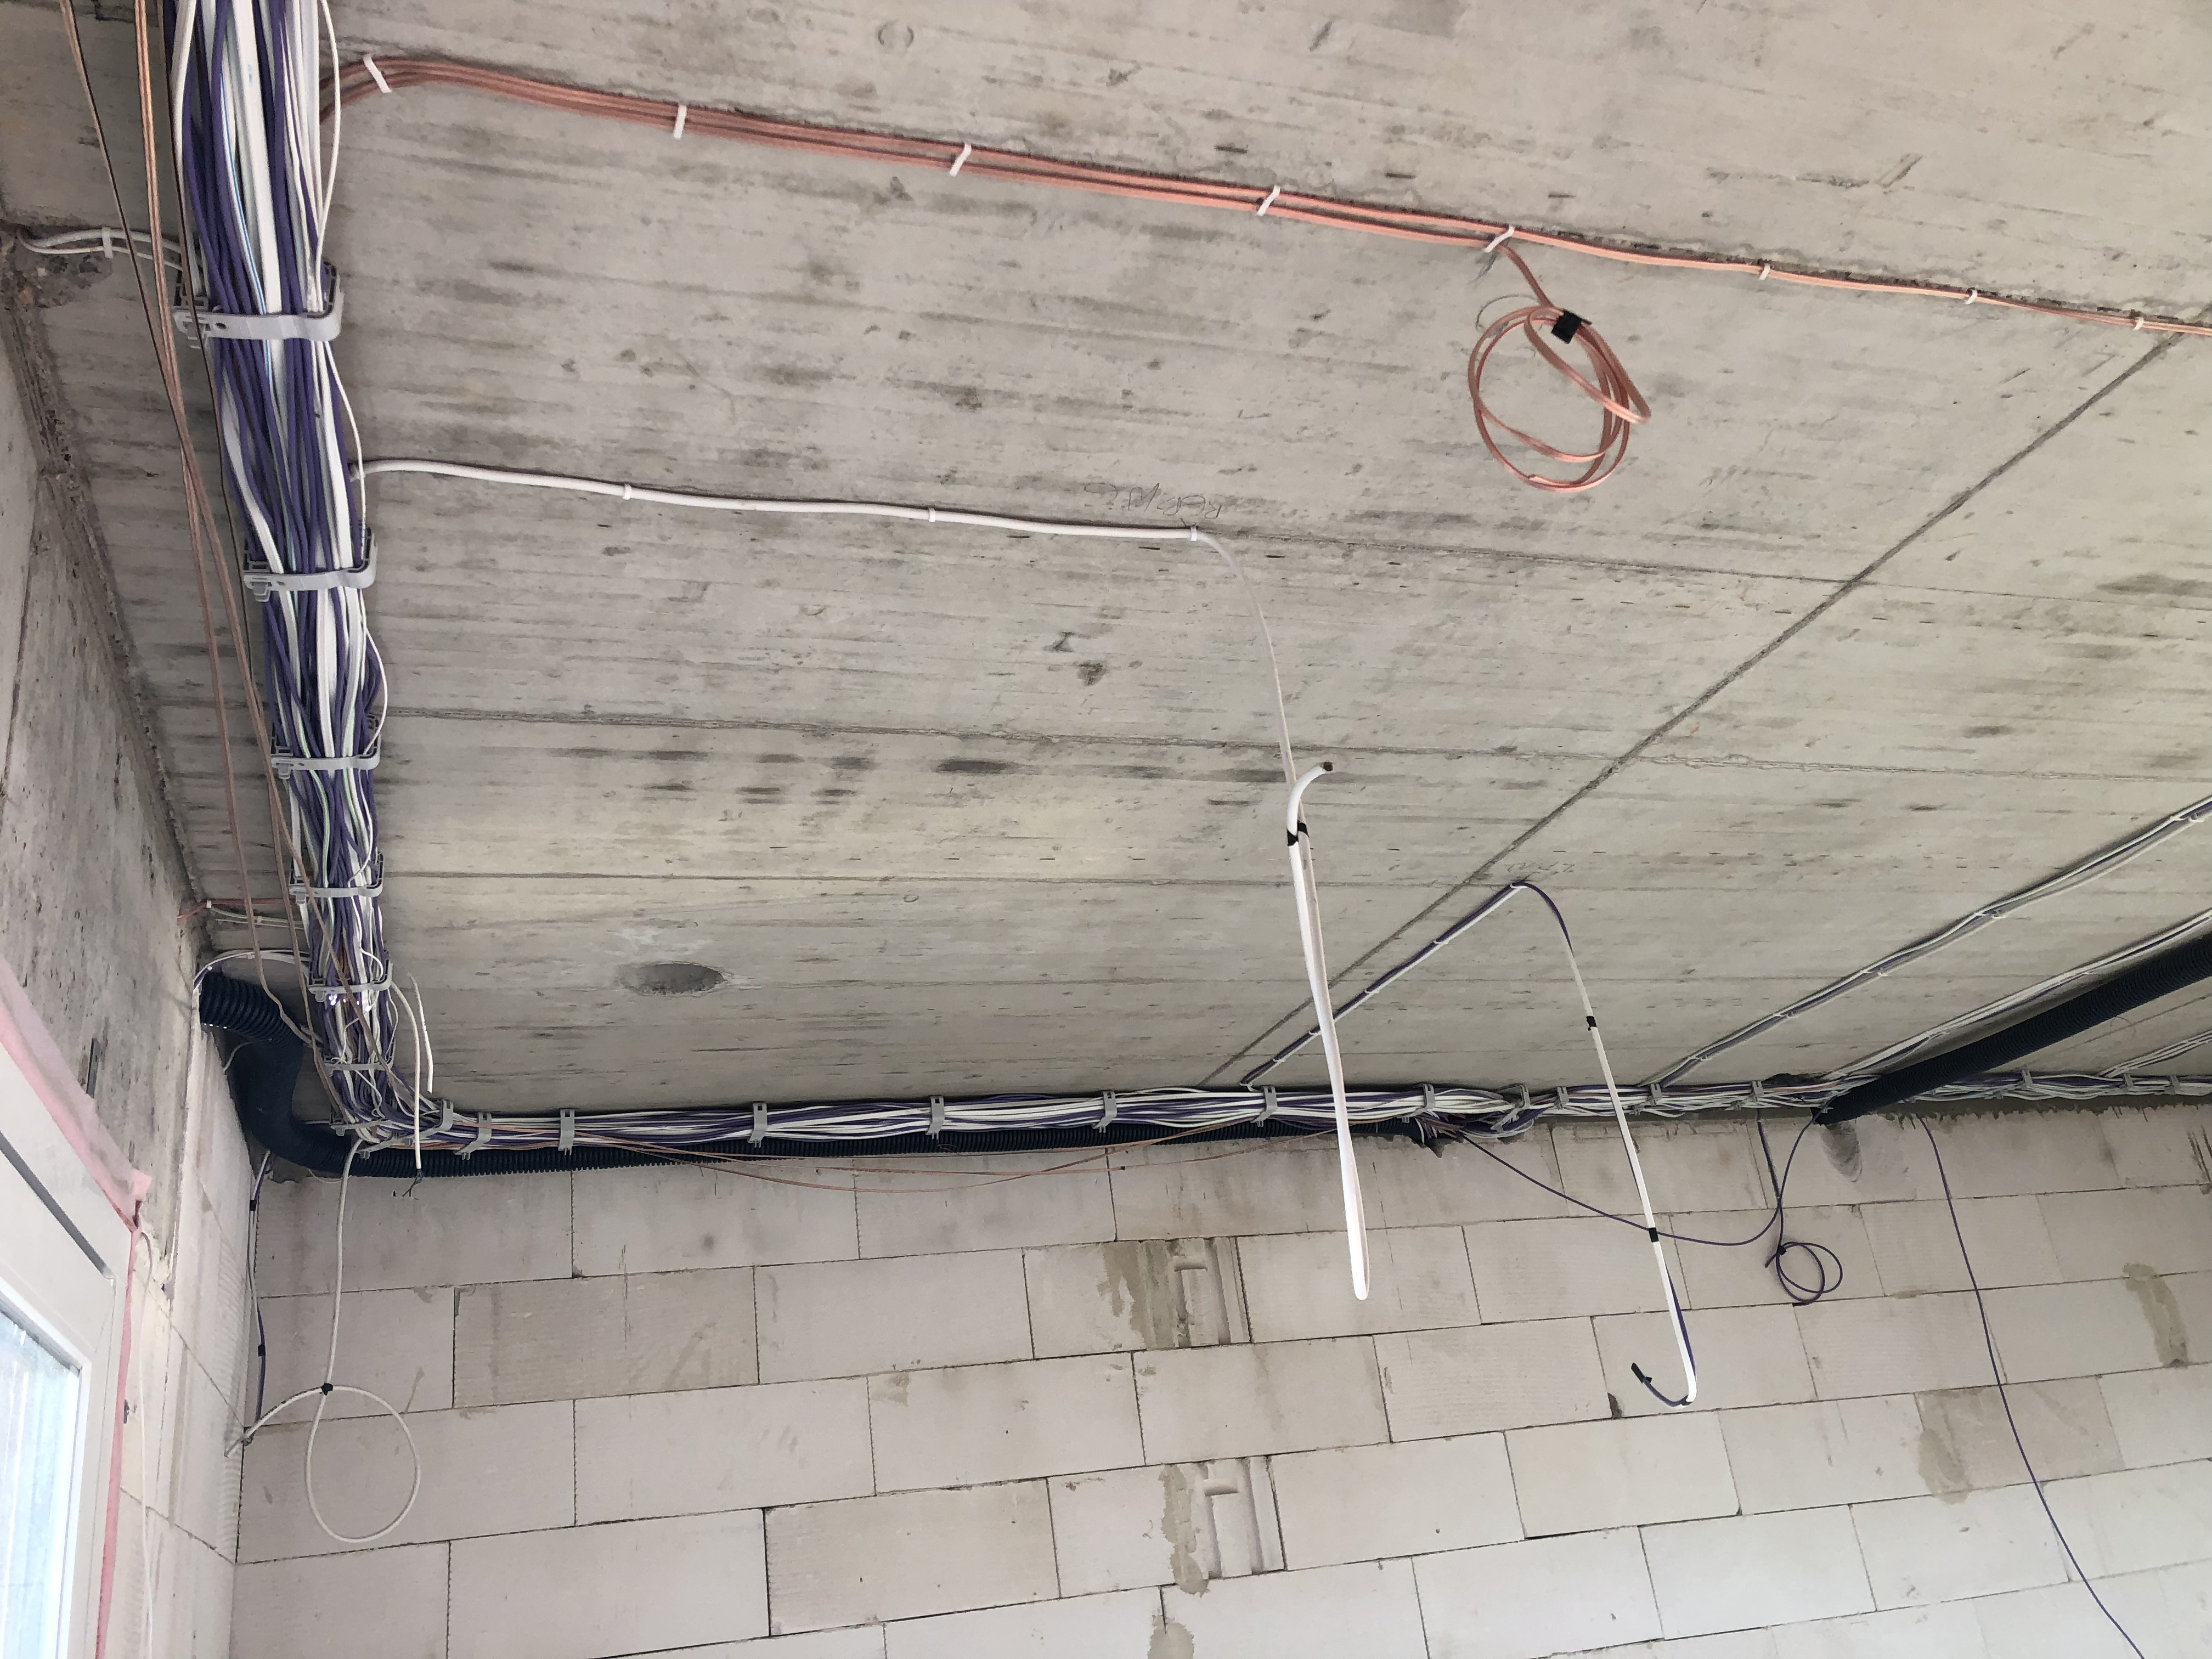
\includegraphics[width=0.8\columnwidth]{imgs/domkable.png}
\caption{Zdjęcie x. Raspberry Pi 4B [źródło: ] \label{rp4b}}
\quad
\end{figure}

Specyfikacja techniczna

\begin{itemize}
	\item Pamięć RAM - 1GB, 2GB lub 4GB LPDDR4
	\item Procesor - Broadcom BCM2711, quad-core Cortex-A72 (ARM v8) 64-bit SoC @ 1.5GHz
	\item GPIO - 2 x 20 pin, raster 2,54 mm (wstecznie kompatybilne)
	\item Łączność \textcolor{blue}{danych}
		\begin{itemize}
			\item 2.4 GHz \textcolor{blue}{oraz} 5.0 GHz IEEE 802.11b/g/n/ac
			\item LAN \textcolor{red}{Gigabit Ethernet}
			\item Bluetooth 5.0
			\item \textcolor{red}{BLE}
			\item 2 × USB 3.0
			\item 2 × USB 2.0
		\end{itemize}
	\item Obraz i dźwięk - 2 × microHDMI (wsparcie 4k)
	\item \textcolor{blue}{Złącza
		\begin{itemize}
			\item DSI dla wyświetlaczy
			\item CSI dla kamer
			\item \textcolor{red}{ Komunikacja - UART, SPI, I2C, GPIO}
		\end{itemize}}
	\item \textcolor{blue}{Multimedia
		\begin{itemize}
			\item H.265 (4Kp60 decode)
			\item H.264 (1080p60 decode, 1080p30 encode)
			\item OpenGL ES, 3.0 graphics
		\end{itemize}}
	\item Karta pamięci - microSD
	\item Systemy operacyjne - Linux Raspbian
	\item Temperatura pracy - 0–50°C
	\item Zasilanie - złącze USB C minimum 5V/3A, złącza GPIO minimum 5V/3A
PoE przy zastosowaniu dedykowanej nakładki
	\item Wymiary - 85 x 56 x 17 mm
\end{itemize}

\subsection{Głośnik jako element wyjściowy}

W zakresie komunikatów głosowych w projekcie został zastosowany głośnik LOGIC CONCEPT LS-09.

Logic Concept LS-09, to zestaw dwóch głośników, które można podłączyć zarówno do komputerów stacjonarnych, laptopów, jak i różnego rodzaju urządzeń multimedialnych. Głośniki charakteryzują się niewielkimi rozmiarami, co było jednym z warunków niezbędnych do realizacji projektu.

Każdy głośnik o mocy 3W. Dzięki niewielkim rozmiarom oraz lekkiej konstrukcji w łatwy i wygodny sposób można je przetransportować.

Zasilane realizowane jest poprzez kabel USB \textcolor{blue}{podłączany do Raspberry pi}.

\begin{figure}[!ht]%
\centering
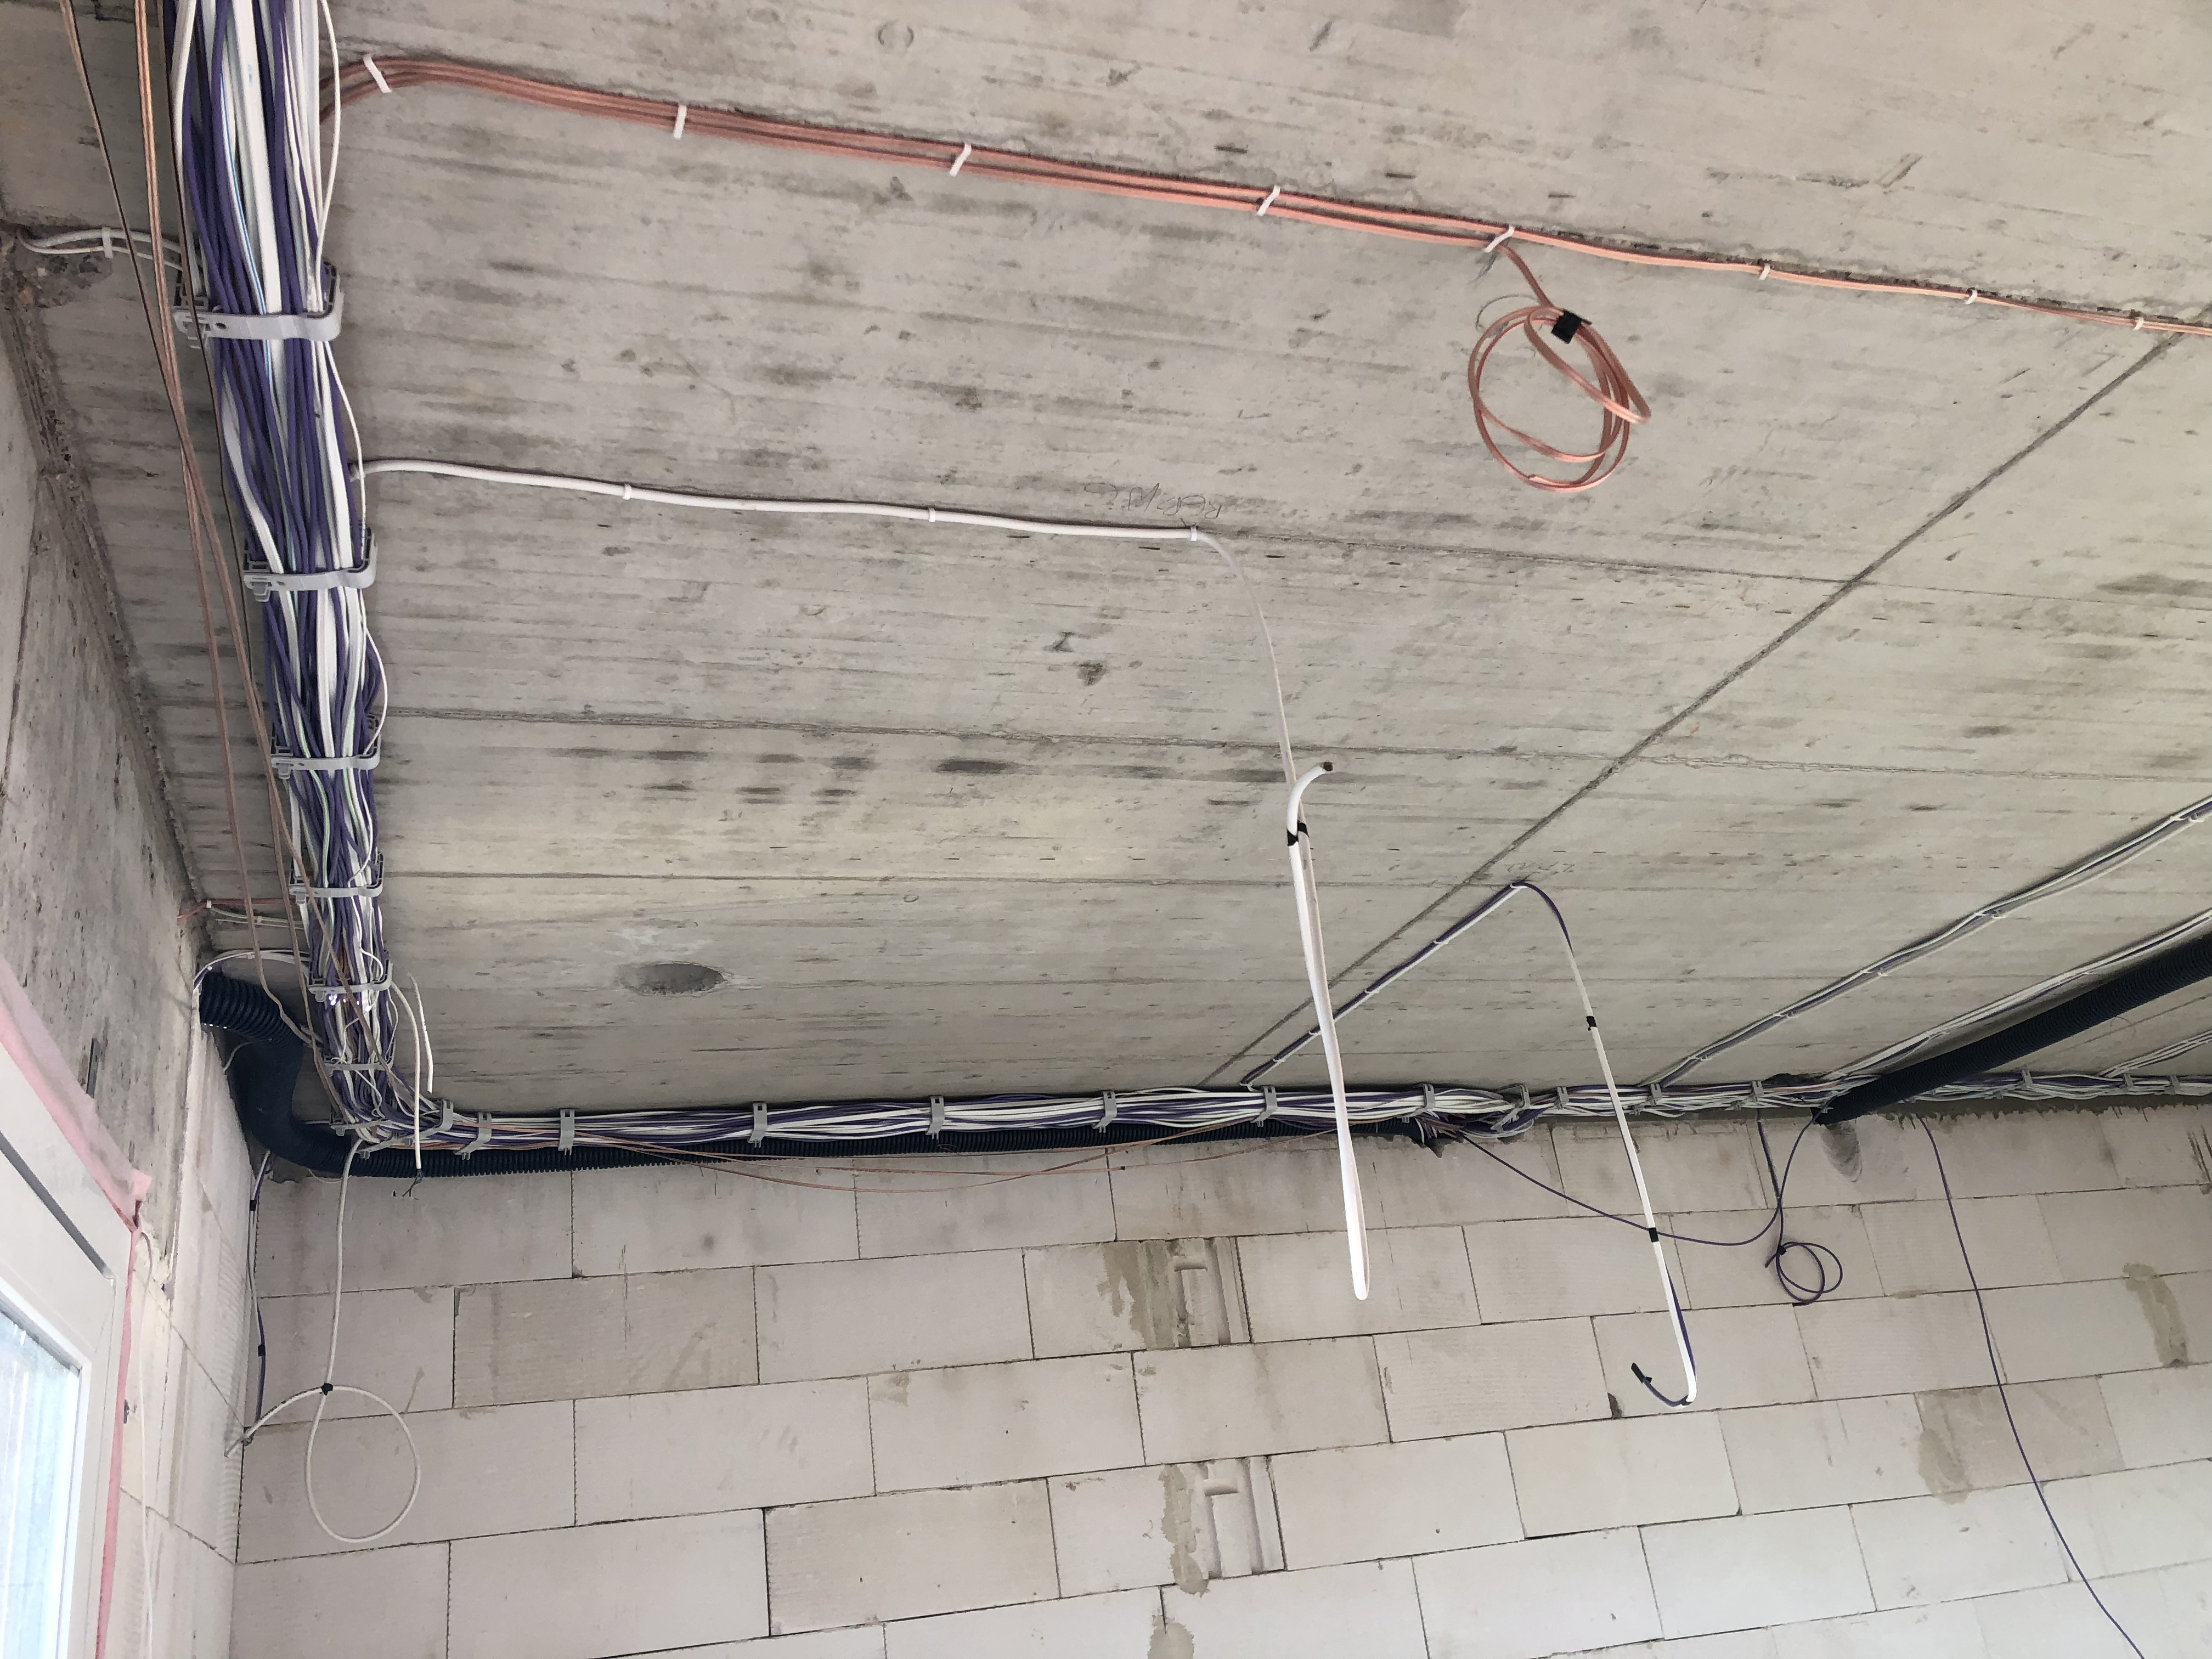
\includegraphics[width=0.8\columnwidth]{imgs/domkable.png}
\caption{Zdjęcie x. Głośniki LOGIC CONCEPT LS-09 [źródło: ] \label{glosnik}}
\quad
\end{figure}

\subsection{Ekran jako element wyjściowy}

W projekcie został zastosowany ekran Ekran dotykowy Waveshare 9904. Jest to ekran rezystancyjny LCD TFT o przekątnej 3,5'' i rozdzielczości 320x480px kompatybilny z Raspberry Pi 4/3/2/B+/Zero.

Oprogramowanie ekranu dotykowego przygotowane przez producenta zawiera sterownikami.

\begin{figure}[!ht]%
\centering
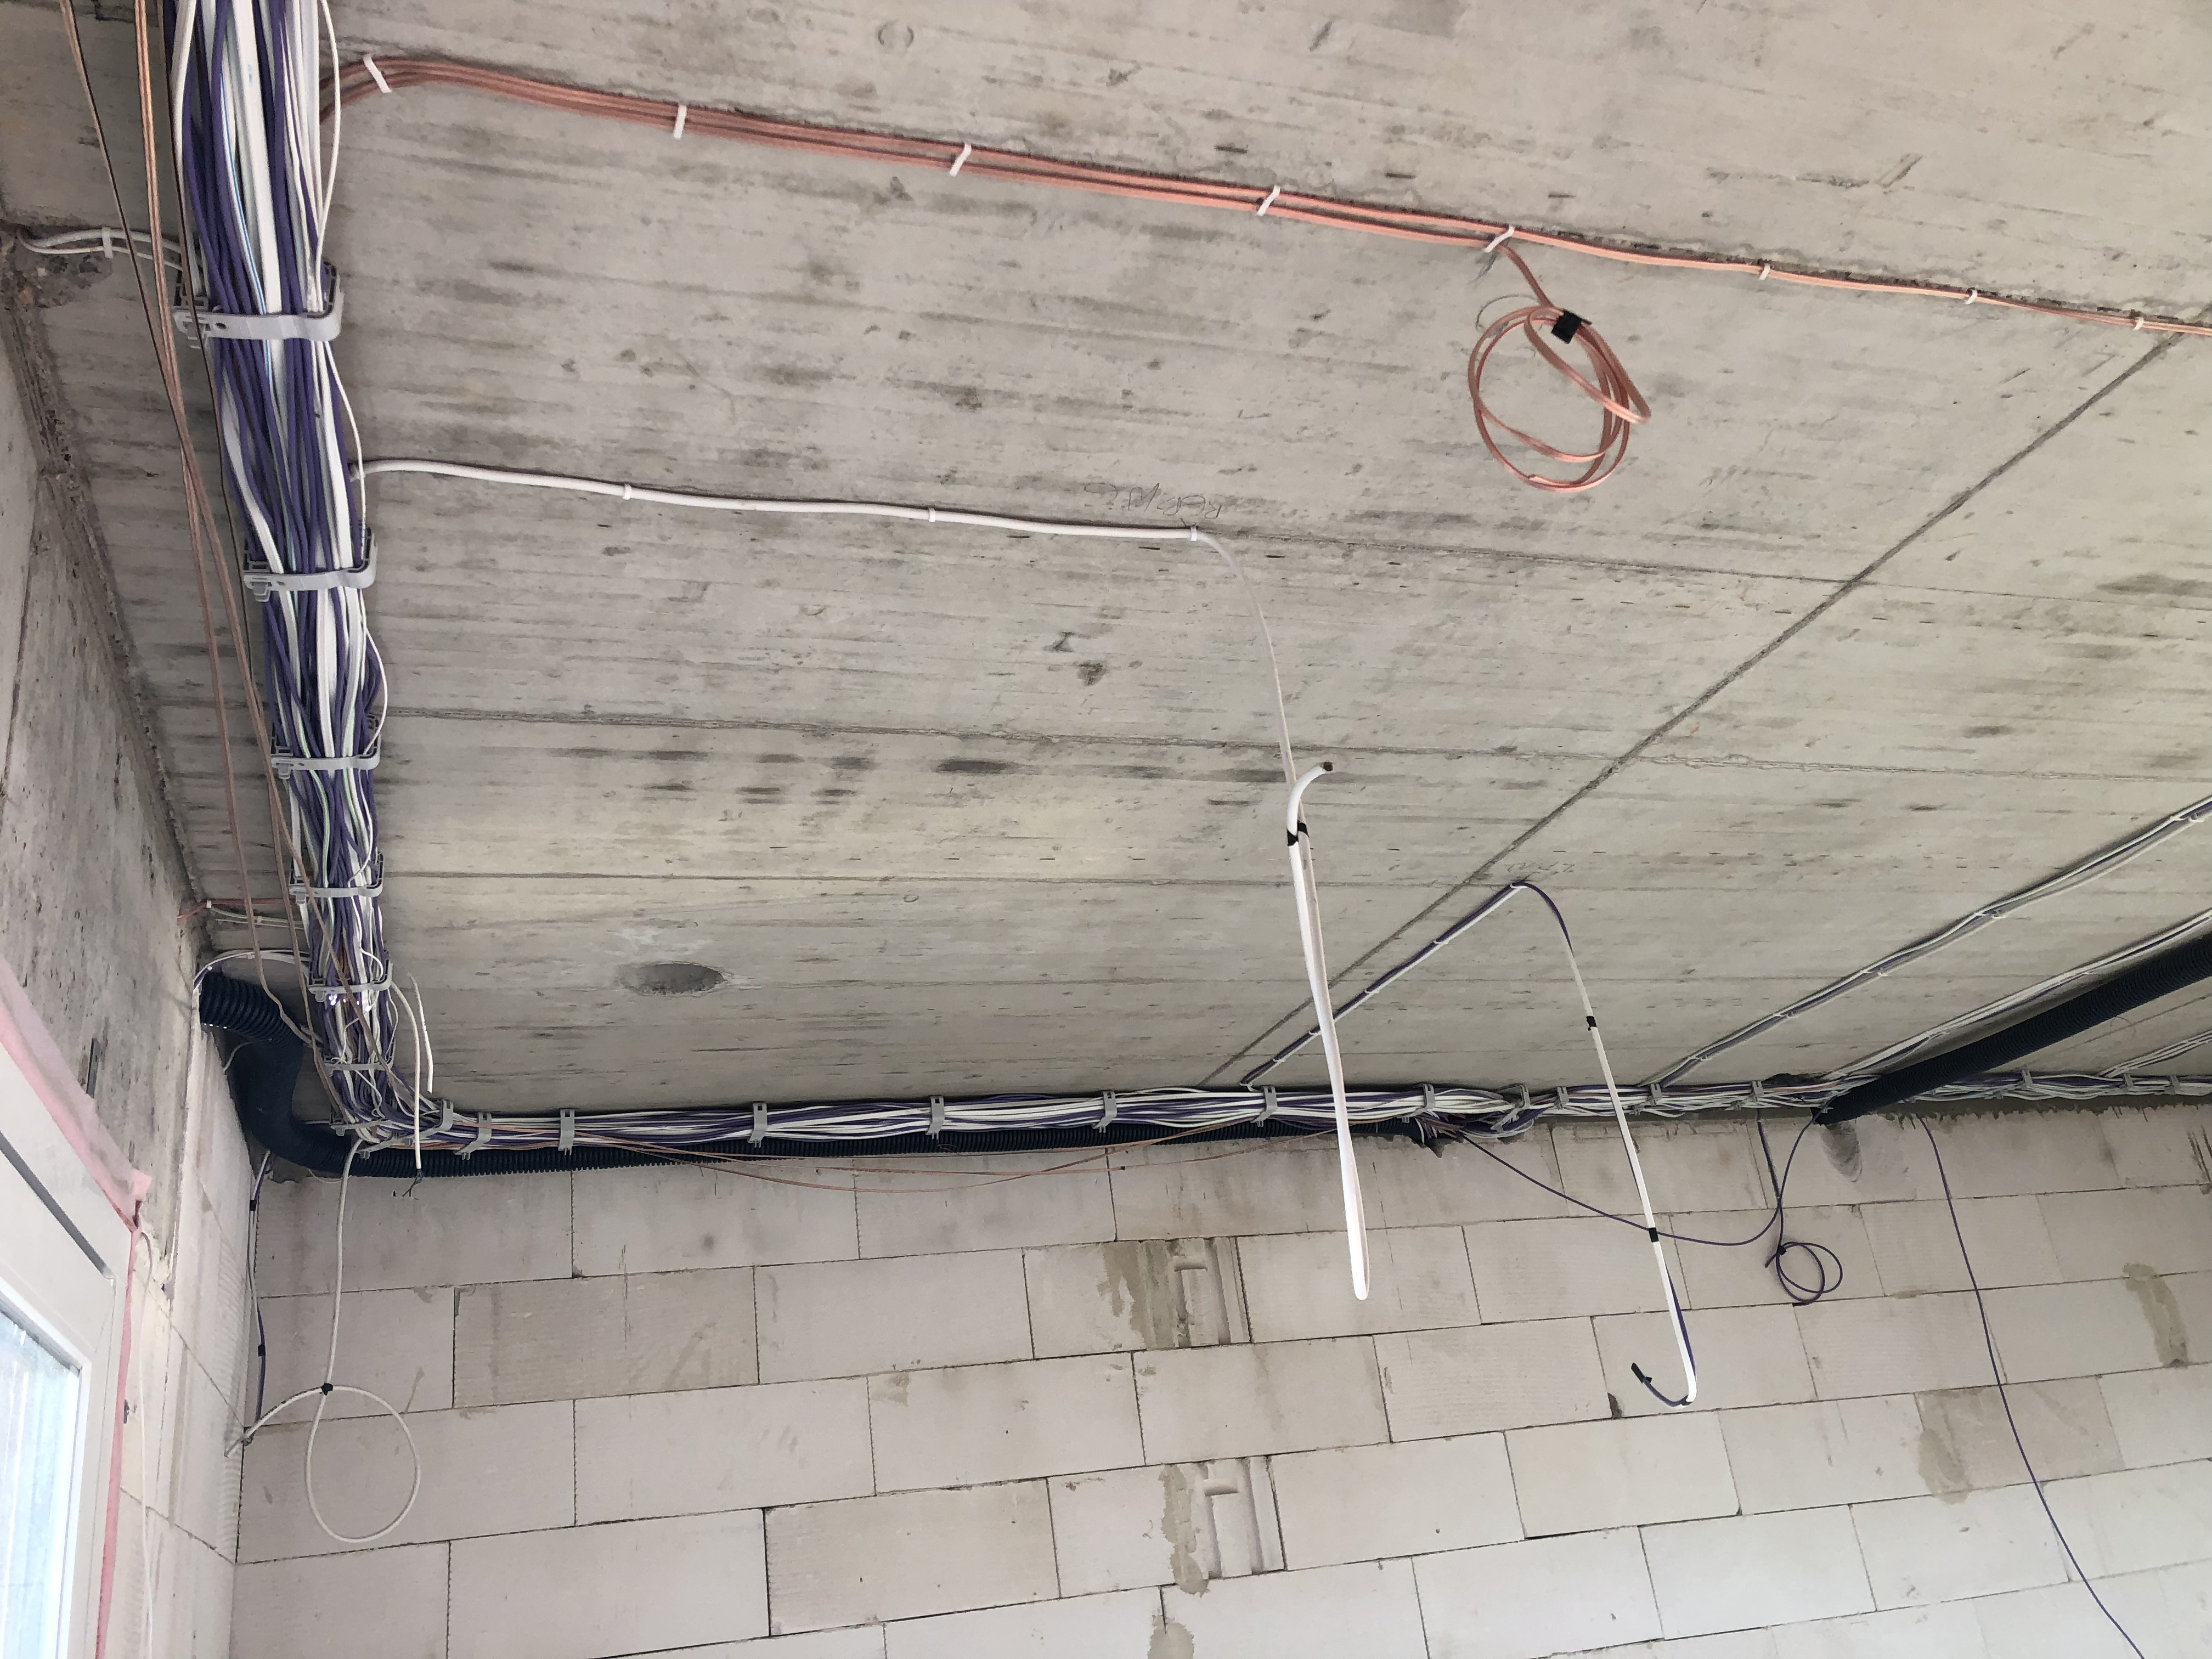
\includegraphics[width=0.8\columnwidth]{imgs/domkable.png}
\caption{Zdjęcie x. Ekran Waveshare 9904 [źródło: ] \label{ekran}}
\quad
\end{figure}

Specyfikacja ekranu dotykowego Waveshare

\begin{itemize}
	\item Typ: ekran dotykowy, rezystancyjny
	\item Przekątna: 3.5"
	\item Rozdzielczość: 320px x 480px
	\item Komunikacja SPI
	\item Współpracuje z: Raspberry Pi w wersji 4B, 3B+, 3B, 2B, B+, Zero i Zero
	\item Wymiary ekranu: 85mm x 56.5mm
\end{itemize}

\subsection{Radiatory}

W celu odprowadzenia ciepła z podzespołów został zastosowany zestaw radiatorów do Raspberry Pi - z taśmą termoprzewodzącą.

Radiatory zbudowane są ze stopów metali dobrze przewodzących ciepło. Ich powierzchnia od strony zewnętrznej jest rozwinięta w postaci żeber.

\subsection{Wentylator}

W celu poprawienia parametrów cieplnych projektu zastosowano w projekcie wymuszony obieg powietrza. W projekcie zastosowano \textcolor{red}{...}

\newpage
\section{Warstwa programistyczna}
\subsection{Python jako język programowania}
\subsection{Biblioteki}
\subsection{Algorytm}
\subsection{Kod}

\newpage
\section{Warstwa produktowa}
\subsection{Technologia druku 3D}
\subsection{Projekt obudowy}
\subsection{Wykonanie obudowy}

\newpage
\section{Realizacja projektu}
\subsection{Napotkane problemy}
\subsection{Możliwości rozbudowy}

\newpage
\section{Wnioski}

\newpage

\bibliographystyle{plain}
\bibliography{praca_dyplomowa_krzysztof_kukiz}


\newpage

\begin{equation} 
\rho\left(\frac{\partial\vec v}{\partial t}+(\vec v\cdot\nabla)\vec v\right) =\rho\vec f - \nabla p + \mu\triangle\vec v, \label{rownanie}
\end{equation} 

\begin{figure}[!ht]%
\centering
\includegraphics[scale=0.85]{logo.eps}
\caption{Podpis rysunku, który jest obrazem wektorowym (EPS). \label{logotyp}}
\qquad
\end{figure}   

\begin{figure}[!ht]%
\centering
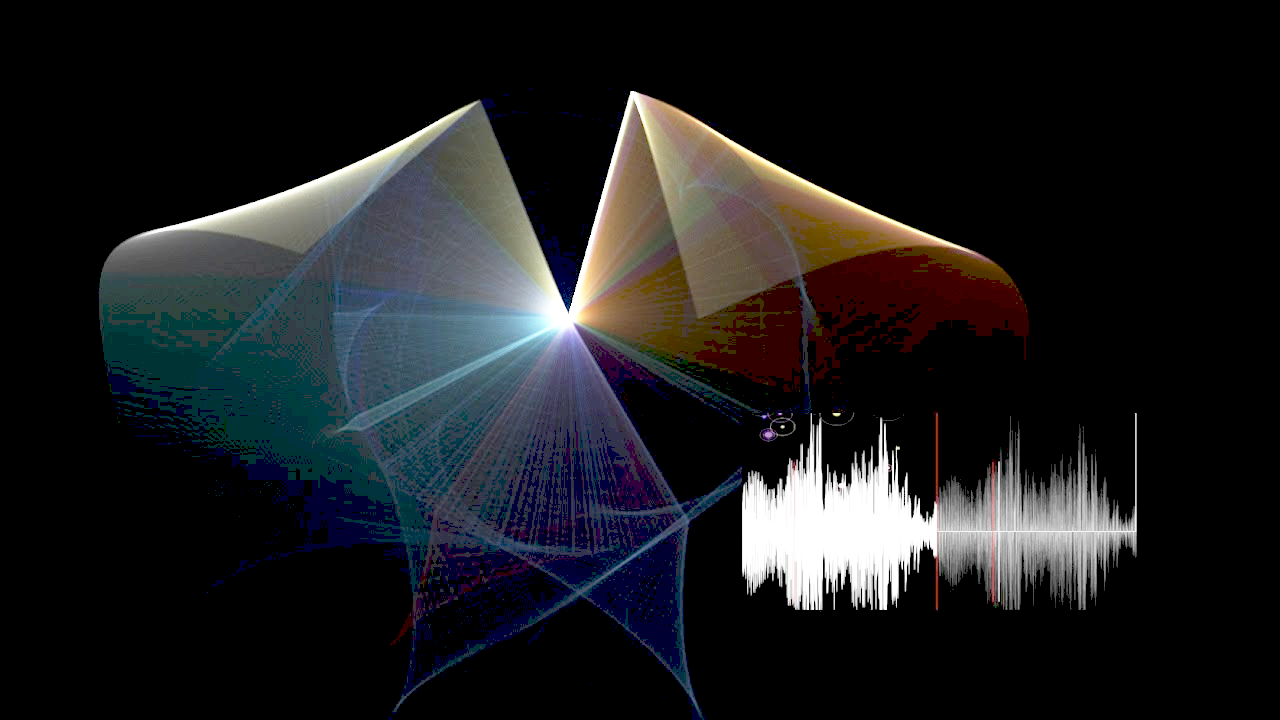
\includegraphics[width=0.8\columnwidth]{pendulums.png}
\caption{To jest rysunek drugi, kilkadziesiąt wahadeł podwójnych z syntezą dźwięku.\label{wahadla}}%
%
\qquad
\end{figure} 

\end{document}




